\chapter{过程管理}

\section{Scrum过程总览}

\subsection{Scrum工作流图}
\begin{figure}[H]
    \centering
    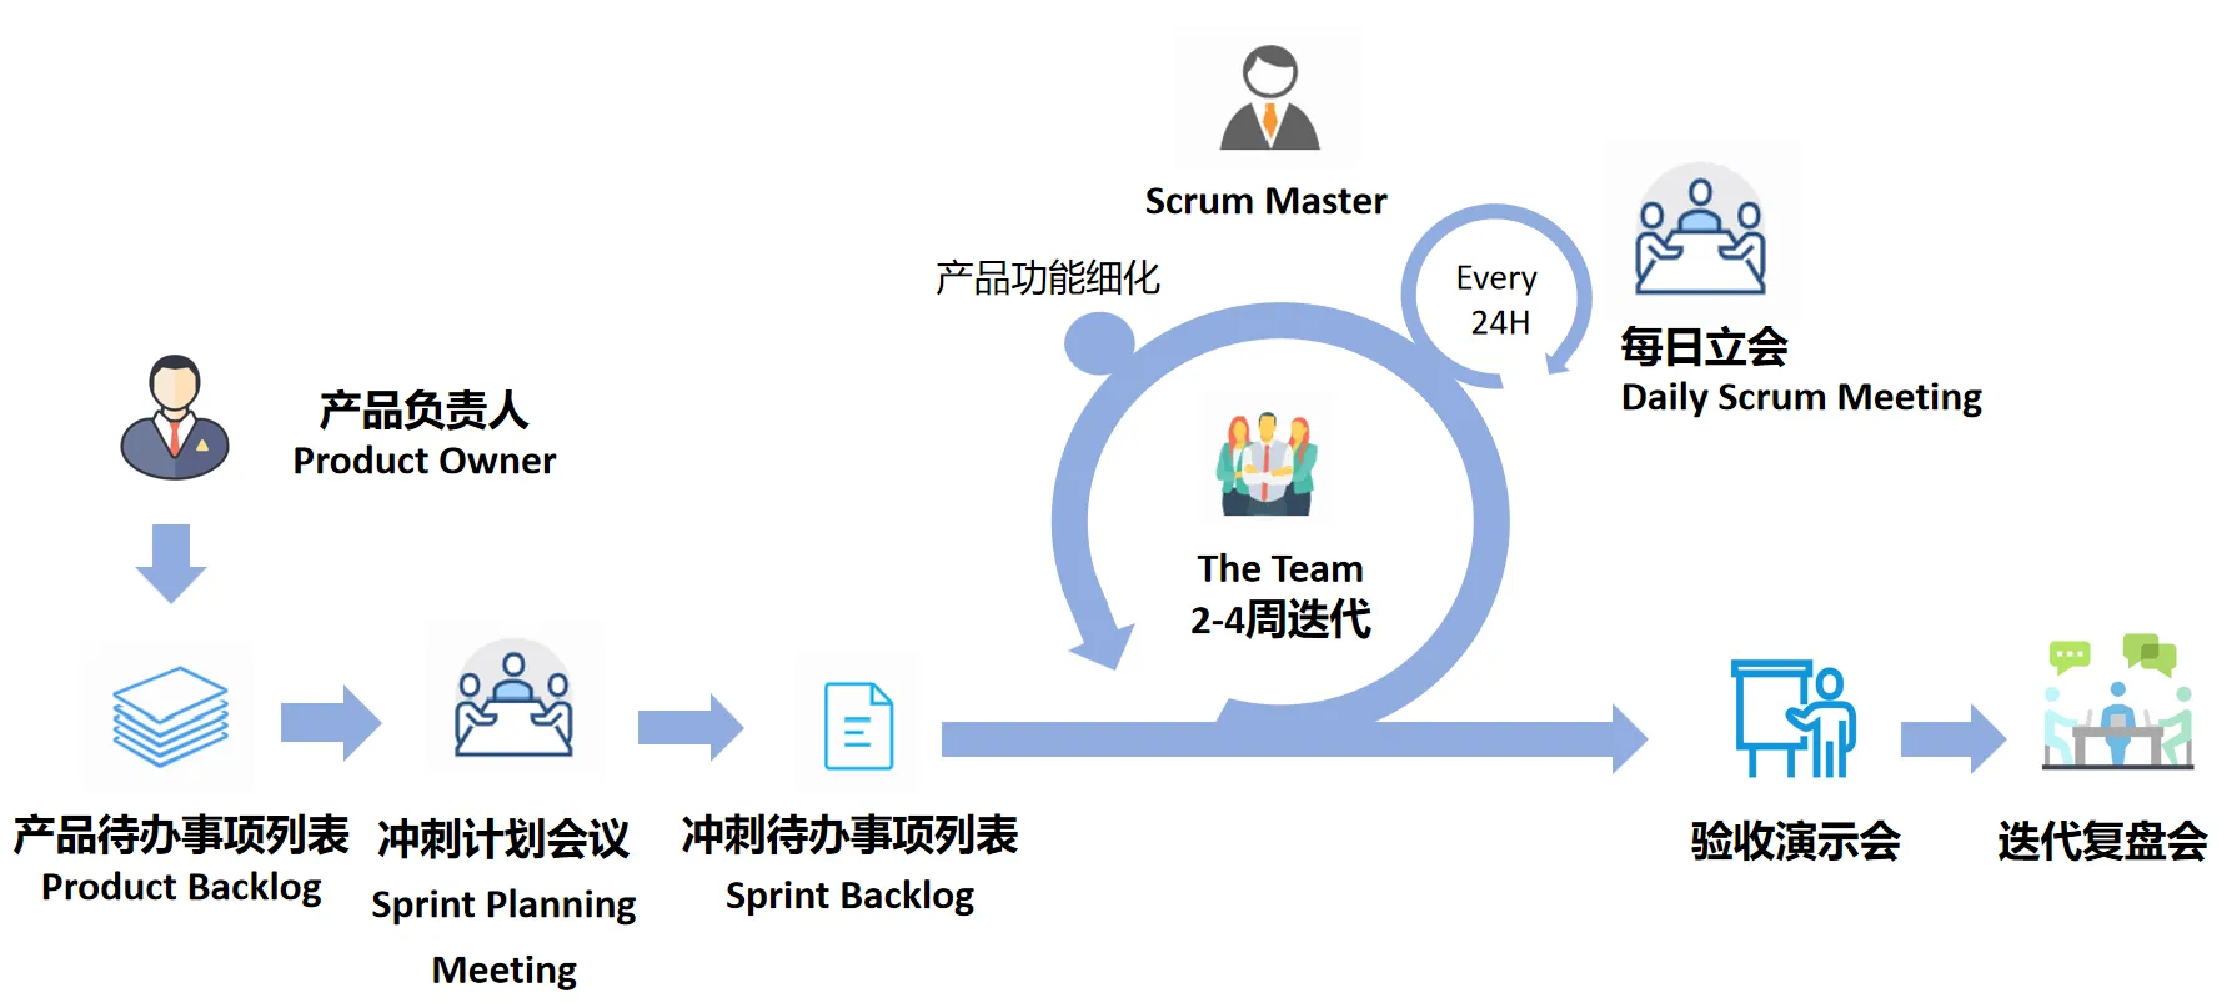
\includegraphics[width=1\textwidth]{figures/in/scrum}
    \caption{Scrum工作流图}
\end{figure}


\subsection{Scrum角色职责重申}
本项目采用 Scrum 敏捷流程，为确保迭代高效进行，各角色在过程管理中的核心职责定义如下：

\begin{enumerate}
    \item \textbf{Product Owner (PO)}
          \begin{itemize}
              \item \textbf{核心动作：} 主持 Sprint 规划会（定义用户故事与优先级）、主持评审会（验收 Sprint 增量）、维护并持续更新 Product Backlog。
          \end{itemize}



    \item \textbf{Scrum Master (SM)}
          \begin{itemize}
              \item \textbf{核心动作：} 组织每日站会与回顾会（Retrospective）、记录开发阻碍并协调资源解决（如协调前后端接口标准）、维护 Scrum 看板（Task Board）流动性。
          \end{itemize}



    \item \textbf{开发团队 (Development Team)}
          \begin{itemize}
              \item \textbf{前端开发：} 参与 Sprint 规划（评估 UI/交互任务工时）、每日站会同步界面开发进度、在评审会中演示前端功能。
              \item \textbf{后端开发：} 参与 Sprint 规划（评估逻辑/数据库任务工时）、每日站会同步 API 接口状态、配合前端进行联调与集成。
              \item \textbf{测试团队：} 测试团队在开发过程中将利用 Postman 进行接口测试，并利用 Issue Tracker（如 GitHub Issues 或禅道）进行缺陷的闭环管理。
                    \begin{itemize}
                        \item 参与 Sprint 规划： 协助定义“完成标准”（Definition of Done），并根据需求编写测试用例。
                        \item 过程质量监控： 每日站会通报 Bug 发现与修复情况，跟踪缺陷生命周期。
                        \item 验收与回归： 在 Sprint 结束前执行系统集成测试，确保功能符合验收标准，把控最终发布质量。
                    \end{itemize}
          \end{itemize}

\end{enumerate}

\begin{longtable}{>{\centering\arraybackslash}m{2.5cm} >{\centering\arraybackslash}m{2.2cm} >{\centering\arraybackslash}m{9.3cm}}

    \caption{Scrum角色职责} \label{tab:training}                                                    \\

    \toprule
    \textbf{角色分类 (Role)} & \textbf{具体职能 (Function)} & \textbf{过程管理中的核心动作 (Key Process Actions)} \\
    \midrule
    \endfirsthead

    \multicolumn{3}{c}{{\tablename\ \thetable{} 续表}}                                            \\
    \toprule
    \textbf{角色分类 (Role)} & \textbf{具体职能 (Function)} & \textbf{过程管理中的核心动作 (Key Process Actions)} \\
    \midrule
    \endhead

    \bottomrule
    \endfoot

    Product Owner        & 产品负责人                    &
    1. 主持 Sprint 规划会：定义用户故事（User Story）并确定优先级。 \newline
    2. 主持 Sprint 评审会：负责验收功能增量。 \newline
    3. 维护 Product Backlog：动态调整需求池，确保高价值任务优先开发。                                                  \\


    Scrum Master         & 敏捷教练                     &
    1. 流程把控：组织每日站会（Stand-up）与迭代回顾会（Retrospective）。 \newline
    2. 障碍清除：记录并协调解决开发阻碍（如前后端接口标准不统一问题）。 \newline
    3. 看板维护：确保 Scrum 看板（Task Board）状态实时更新，监控任务流动。                                               \\


    Development Team     & 前端开发                     &
    1. 工时估算：参与规划会，评估 UI/交互类任务的工时。 \newline
    2. 进度同步：每日站会同步界面开发进度，暴露联调风险。 \newline
    3. 演示反馈：在评审会中演示前端可视化的功能模块。                                                                  \\


    Development Team     & 后端开发                     &
    1. 工时估算：参与规划会，评估业务逻辑与数据库任务工时。 \newline
    2. 接口同步：每日站会汇报 API 开发状态，确保接口文档（如 Swagger）及时更新。 \newline
    3. 联调支持：配合前端与测试团队进行集成测试与问题排查。                                                               \\


    Development Team     & 测试团队                     &
    1. 标准制定：参与规划会，协助定义完成标准 (DoD)，编写测试用例。 \newline
    2. 质量监控：每日站会通报 Bug 发现与修复进度，跟踪缺陷生命周期。 \newline
    3. 验收闭环：在 Sprint 结束前执行回归测试，确保交付版本符合验收要求。                                                    \\
\end{longtable}


\section{立项组会}

\subsection{会议快照}

\begin{longtable}{>{\centering\arraybackslash}m{1.5cm} >{\centering\arraybackslash}m{11cm} >{\centering\arraybackslash}m{2.5cm} >{\centering\arraybackslash}m{2.5cm}}

    \caption{立项组会会议快照} \label{tab:training}                                        \\

    \toprule
    \textbf{维度} & \textbf{内容}                                                      \\
    \midrule
    \endfirsthead

    \multicolumn{2}{c}{{\tablename\ \thetable{} 续表}}                               \\
    \toprule
    \textbf{维度} & \textbf{内容}                                                      \\
    \midrule
    \endhead

    \bottomrule
    \endfoot

    时间          & 2025 年 10 月 10 日 13:00–15:00                                     \\
    地点          & 郑东图书馆研究生包厢 302 会议室                                               \\
    参会人         & 全体 6 名核心成员：高灿（组长/Scrum Master）、贾思韵（Product Owner）、戴茗静、曾意、杨晓越、任晓华 \\
    目标          &
    1.对齐“12 月 14 日上线 MVP”里程碑； \newline
    2.敲定 3 轮 Sprint 节奏； \newline
    3.锁定 Sprint1 最小可用功能包与工具链。                                                      \\
\end{longtable}

\subsection{核心决议}

\begin{enumerate}
    \item \textbf{迭代节奏}
          \begin{itemize}
              \item 2周~3周 / Sprint，共 3 轮。
              \item 排期：
                    \begin{itemize}
                        \item Sprint1：10-11 ～ 10-30（目标：用户独立完成“发现店铺→下单支付”全链路 MVP）
                        \item Sprint2：10-31 ～ 11-16（目标：商家“开店→接单”完整工作流 + 用户互动）
                        \item Sprint3：11-17 ～ 12-07（目标：管理端治理、AI 客服、性能压测、灰度上线）
                    \end{itemize}
              \item 12-08 ～ 12-14 为“硬上线窗口”：灰度 → 全量 → 项目结项评审。
          \end{itemize}



    \item \textbf{需求优先级}
          \begin{itemize}
              \item 采用 MoSCoW 规则：
                    \begin{itemize}
                        \item Must（P0）：US001、US003、US004（注册、商铺搜、购物车支付）必须进 Sprint1；
                        \item Should（P1）：US005、US006、US007、US008 进 Sprint2；
                        \item Could（P2）：US009～US019 按市场反馈插空实现。
                    \end{itemize}
              \item 现场把 Product Backlog 按故事点（共 77 点）拖入 PingCode，PO（贾思韵）拥有唯一调整权。
          \end{itemize}



    \item \textbf{工具链 & 信息辐射}
          \begin{itemize}
              \item PingCode：需求池 + Sprint 看板 + 燃尽图（自动同步 Git 分支）；
              \item 会议：每日 19:00 15-min 站会；
              \item 腾讯文档：会议纪要、风险看板模板（统一 ID：PBD-2025）；
              \item Postman Team Workspace：接口集合统一命名规范“模块-版本-环境”；
              \item 代码仓库：Gitee 企业版，main 分支保护 + PR 评审必须 2 人通过；
              \item 生产监控：Prometheus + Grafana（曾意负责 10-22 前搭好看板）。
          \end{itemize}

\end{enumerate}


\subsection{即时任务分配（RACI 到人头）}


\begin{longtable}{>{\centering\arraybackslash}m{3.5cm} >{\centering\arraybackslash}m{4cm} >{\centering\arraybackslash}m{2.5cm} >{\centering\arraybackslash}m{3cm}}

    \caption{即时任务分配} \label{tab:training}                                                                    \\

    \toprule
    \textbf{任务}                         & \textbf{负责人}       & \textbf{培训交付时间形式} & \textbf{完成标准}             \\
    \midrule
    \endfirsthead

    \multicolumn{4}{c}{{\tablename\ \thetable{} 续表}}                                                         \\
    \toprule
    \textbf{任务}                         & \textbf{负责人}       & \textbf{培训交付时间形式} & \textbf{完成标准}             \\
    \midrule
    \endhead

    \bottomrule
    \endfoot

    搭建 PingCode 项目骨架 \& 导入 77 点 Backlog & 高灿（Scrum Master）   & 10-10 20:00       & 看板可正常拖拽，燃尽图自动生成           \\
    创建 Sprint1 里程碑 \& 关联 US001/003/004  & 高灿（Tech Lead）      & 10-10 22:00       & 故事状态=待办，估算工时≤8 h/任务       \\
    明确 Sprint1 Sprint Goal 并邮件公告        & 贾思韵（Product Owner） & 10-10 12:00       & 邮件抄送全体，目标可测               \\
    风险看板初始化（含 Top10 风险）                 & 任晓华（QA）            & 10-10 前           & 风险等级、应对、Owner、Deadline 明确 \\
\end{longtable}



\subsection{会议输出物}
\begin{enumerate}
    \item 《立项决议书》PDF（已群邮件，命名：PBD-Kickstart-V1.0-20251020.pdf）
    \item Sprint1 Sprint Backlog 线上看板链接（PingCode 项目 ID：PBD-2025）
    \item 风险看板（腾讯文档）
    \item 会议纪要（腾讯文档）
\end{enumerate}

\subsection{后续跟踪}
\begin{enumerate}
    \item 每日站会由高灿主持，超时 15 min 自动转线下小会；
    \item 每周五 18:00 前在风险看板更新一次状态；
    \item Sprint1 评审会预定 10-31 20:00，届时如未完成 P0 功能，自动触发“紧急回顾”流程。
\end{enumerate}

\section{Sprint迭代管理}

\subsection{Sprint1:用户注册/登录/鉴权 + 订单业务核心流程(10.11-10.30)}
\begin{levellist}
    \item \textbf{Sprint 规划会记录}
    \begin{itemize}
        \item 会议时间：2025年10月11日 19:00-20:30
        \item 参会人员：全体成员（Product Owner贾思韵主导，前后端共同估算工时）
        \item Sprint 目标：构建用户从发现店铺到完成支付的全链路购物体验，支持用户独立完成首次下单，交付系统最小可用版本。
        \item Sprint Backlog（前后端任务整合，关联用户故事）：

              \begin{longtable}{>{\centering\arraybackslash}m{1.4cm} >{\centering\arraybackslash}m{3.1cm} >{\centering\arraybackslash}m{1.7cm} >{\centering\arraybackslash}m{1.8cm} >{\centering\arraybackslash}m{1.8cm} >{\centering\arraybackslash}m{1.3cm} >{\centering\arraybackslash}m{1.2cm}}

                  \caption{Sprint1前后端任务整合与关联用户故事} \label{tab:training}                                                                              \\

                  \toprule
                  \textbf{任务ID} & \textbf{任务名称}               & \textbf{关联用户故事} & \textbf{负责成员} & \textbf{预估工时(小时)} & \textbf{依赖关系} & \textbf{任务状态} \\
                  \midrule
                  \endfirsthead

                  \multicolumn{7}{c}{{\tablename\ \thetable{} 续表}}                                                                                  \\
                  \toprule
                  \textbf{任务ID} & \textbf{任务名称}               & \textbf{关联用户故事} & \textbf{负责成员} & \textbf{预估工时(小时)} & \textbf{依赖关系} & \textbf{任务状态} \\
                  \midrule
                  \endhead

                  \bottomrule
                  \endfoot


                  T101-1        & 用户表设计与注册接口开发                & US001           & 戴茗静           & 3                 & 无             & 待办            \\
                  T101-2        & 登录接口与JWT token签发            & US001           & 戴茗静           & 3                 & 依赖T101-1      & 待办            \\
                  T101-3        & Spring Security配置与token验证   & US001           & 戴茗静           & 2                 & 依赖T101-2      & 待办            \\
                  T102-1        & Login.vue登录页面开发             & US001           & 杨晓越           & 4                 & 无             & 待办            \\
                  T102-2        & Register.vue注册页面开发          & US001           & 杨晓越           & 4                 & 无             & 待办            \\
                  T102-3        & 前端路由守卫实现                    & US001           & 杨晓越           & 3                 & 依赖T101-2      & 待办            \\
                  T103-1        & business表设计与基础查询接口          & US002           & 曾意            & 3                 & 无             & 待办            \\
                  T103-2        & 商铺分类筛选接口开发                  & US002           & 曾意            & 2                 & 依赖T103-1      & 待办            \\
                  T103-3        & 商铺关键字搜索接口开发                 & US002           & 曾意            & 2                 & 依赖T103-1      & 待办            \\
                  T103-4        & 首页轮播推荐接口开发                  & US002           & 曾意            & 2                 & 依赖T103-1      & 待办            \\
                  T104-1        & Index.vue首页框架开发             & US002           & 贾思韵           & 4                 & 无             & 待办            \\
                  T104-2        & 分类入口与搜索栏组件                  & US002           & 贾思韵           & 2                 & 依赖T104-1      & 待办            \\
                  T104-3        & 轮播推荐与筛选组件                   & US002           & 贾思韵           & 2                 & 依赖T103-4      & 待办            \\
                  T105-1        & 商铺详情查询接口开发                  & US003           & 曾意            & 3                 & 依赖T103-1      & 待办            \\
                  T105-2        & 商品列表查询接口开发                  & US003           & 曾意            & 3                 & 依赖food表设计     & 待办            \\
                  T106-1        & BusinessInfo.vue商铺详情页框架     & US003           & 贾思韵           & 4                 & 依赖T105-1      & 待办            \\
                  T106-2        & 商品列表组件开发                    & US003           & 贾思韵           & 4                 & 依赖T105-2      & 待办            \\
                  T107-1        & delivery\_address表设计与CRUD接口 & US004           & 高灿            & 5                 & 无             & 待办            \\
                  T107-2        & 手机号双重验证逻辑                   & US004           & 高灿            & 3                 & 无             & 待办            \\
                  T108-1        & UserAddress.vue地址列表页        & US004           & 杨晓越           & 3                 & 依赖T107-1      & 待办            \\
                  T108-2        & 新增与编辑地址页面                   & US004           & 杨晓越           & 3                 & 依赖T108-1      & 待办            \\
                  T109-1        & cart表设计与购物车接口               & US005           & 戴茗静           & 4                 & 依赖food表       & 待办            \\
                  T109-2        & orders表设计与订单创建接口            & US005           & 戴茗静           & 4                 & 依赖T109-1      & 待办            \\
                  T109-3        & 订单总价计算逻辑                    & US005           & 戴茗静           & 5                 & 依赖T109-2      & 待办            \\
                  T109-4        & 支付方式接口对接                    & US005           & 戴茗静           & 5                 & 依赖T109-2      & 待办            \\
                  T110-1        & 商铺详情页购物车组件                  & US005           & 贾思韵           & 3                 & 依赖T106-1      & 待办            \\
                  T110-2        & Cart.vue购物车页面开发             & US005           & 贾思韵           & 3                 & 依赖T109-1      & 待办            \\
                  T110-3        & Payment.vue支付页面开发           & US005           & 贾思韵           & 3                 & 依赖T109-2      & 待办            \\
                  T111-1        & 订单列表查询接口开发                  & US007           & 戴茗静           & 3                 & 依赖orders表     & 待办            \\
                  T111-2        & 订单详情查询接口开发                  & US007           & 戴茗静           & 3                 & 依赖T111-1      & 待办            \\
                  T112-1        & Order.vue订单列表页开发            & US007           & 杨晓越           & 3                 & 依赖T111-1      & 待办            \\
                  T112-2        & 订单详情与取消功能                   & US007           & 杨晓越           & 2                 & 依赖T111-2      & 待办            \\
                  T113-1        & WebSocket服务搭建               & US015           & 曾意            & 3                 & 无             & 待办            \\
                  T113-2        & 订单状态推送逻辑                    & US015           & 曾意            & 5                 & 依赖T111-1      & 待办            \\
                  T114-1        & WebSocket客户端集成              & US015           & 杨晓越           & 5                 & 依赖T113-1      & 待办            \\
                  T114-2        & 消息接收与展示组件                   & US015           & 杨晓越           & 3                 & 依赖T113-2      & 待办            \\
                  T115-1        & 前后端接口联调                     & -               & 任晓华           & 5                 & 依赖所有接口完成      & 待办            \\
                  T115-2        & 功能集成测试                      & -               & 任晓华           & 5                 & 依赖T115-1      & 待办            \\
              \end{longtable}

        \item 总工时与里程碑：
              \begin{itemize}
                  \item 总工时：128小时（前端61小时，后端67小时）
                  \item 关键里程碑：
                        \begin{enumerate}
                            \item 10月15日前：完成用户认证和商铺查询接口。
                            \item 10月20日前：完成购物车和订单核心接口。
                            \item 10月25日前：完成前后端联调。
                            \item 10月30日：Sprint结束，交付最小可用版本。
                        \end{enumerate}

              \end{itemize}

    \end{itemize}

    \item \textbf{每日站会记录}

    \begin{longtable}{>{\centering\arraybackslash}m{1cm} >{\centering\arraybackslash}m{1cm} >{\centering\arraybackslash}m{8.5cm} >{\centering\arraybackslash}m{3cm}}

        \caption{Sprint1每日站会记录} \label{tab:training}                                                                                                                                                                                                     \\

        \toprule
        \textbf{日期}                                         & \textbf{参会人员}                                                                    & \textbf{核心内容}                                                                          & \textbf{阻碍与解决} \\
        \midrule
        \endfirsthead

        \multicolumn{4}{c}{{\tablename\ \thetable{} 续表}}                                                                                                                                                                                                 \\
        \toprule
        \textbf{日期}                                         & \textbf{参会人员}                                                                    & \textbf{核心内容}                                                                          & \textbf{阻碍与解决} \\
        \midrule
        \endhead

        \bottomrule
        \endfoot


        10月11日                                              & 全体                                                                               & - 高灿：今天召开Sprint启动会；无阻碍 \newline
        - 贾思韵：昨天整理需求文档；今天进行详细任务分解；无阻碍 \newline
        - 全体：确认Sprint目标为7个用户故事，总计39故事点                      & 状态：Sprint1正式启动，任务分解完成                                                                                                                                                                      \\

        10月12日                                              & 全体                                                                               & - 戴茗静：昨天分析用户认证技术方案；今天开始T101-1用户表设计与注册接口开发；无阻碍 \newline
        - 曾意：昨天分析商铺查询需求；今天开始T103-1 business表设计与基础查询接口；无阻碍 \newline
        - 杨晓越：昨天搭建前端项目框架；今天开始T102-1 Login.vue登录页面开发；无阻碍     & 无阻碍 - 项目启动，数据库设计和页面框架并行开发                                                                                                                                                                  \\


        10月13日                                              & 全体                                                                               & - 戴茗静：昨天完成T101-1用户表设计；今天开发注册接口BCrypt加密逻辑；无阻碍 \newline
        - 杨晓越：昨天完成T102-1登录页面框架；今天完善表单校验和样式；无阻碍 \newline
        - 曾意：昨天完成T103-1 business表设计；今天开发基础查询接口；无阻碍 \newline
        - 高灿：昨天分析地址管理需求；今天开始T107-1 delivery\_address表设计；无阻碍 & 进度：数据库设计按计划进行                                                                                                                                                                              \\
        10月14日                                              & 全体                                                                               & - 戴茗静：昨天完成注册接口开发；今天开始T101-2登录接口与JWT token签发；无阻碍 \newline
        - 杨晓越：昨天完成T102-1登录页面开发；今天开始T102-2 Register.vue注册页面开发；无阻碍 \newline
        - 曾意：昨天完成基础查询接口；今天开始T103-2商铺分类筛选接口开发；无阻碍 \newline
        - 贾思韵：昨天分析首页需求；今天开始T104-1 Index.vue首页框架开发；无阻碍       & 进度：用户认证功能开发过半                                                                                                                                                                              \\
        10月15日                                              & 全体                                                                               & - 戴茗静：昨天完成T101-2登录接口核心逻辑；今天开发T101-3 Spring Security配置与token验证；阻碍：token刷新机制需确认 \newline
        - 杨晓越：昨天完成T102-2注册页面布局；今天实现密码强度校验和确认密码功能；无阻碍 \newline
        - 曾意：昨天完成T103-2分类筛选接口；今天开始T103-3商铺关键字搜索接口；无阻碍 \newline
        - 贾思韵：昨天完成T104-1首页框架；今天开发分类入口组件；无阻碍                 & 阻碍：token刷新机制 \newline
        解决：与高灿讨论确定采用refresh token方案                                                                                                                                                                                                                      \\
        10月16日                                              & 全体                                                                               & - 戴茗静：昨天研究token刷新方案；今天实现refresh token逻辑；阻碍：方案讨论耗时 \newline
        - 杨晓越：昨天完成T102-2注册页面功能；今天开发T102-3前端路由守卫；无阻碍 \newline
        - 曾意：昨天完成T103-3关键字搜索接口；今天优化搜索算法性能；无阻碍 \newline
        - 高灿：昨天完成T107-1地址表设计；今天开发CRUD接口；无阻碍                 & 阻碍：token刷新机制技术方案未确定 \newline
        影响：T101-3延误1小时 \newline
        解决：Scrum Master组织技术讨论确定方案                                                                                                                                                                                                                        \\
        10月17日                                              & 全体                                                                               & - 戴茗静：昨天确定refresh token方案；今天完成T101-3 Spring Security配置；无阻碍 \newline
        - 杨晓越：昨天完成T102-3路由守卫基础功能；今天优化登录状态管理；无阻碍 \newline
        - 曾意：昨天完成搜索接口优化；今天开发T103-4首页轮播推荐接口；无阻碍 \newline
        - 贾思韵：昨天完成分类入口组件；今天开发T104-2搜索栏组件；无阻碍                & 进度：token问题解决，用户认证功能基本完成                                                                                                                                                                    \\
        10月18日                                              & 全体                                                                               & - 戴茗静：昨天完成T101-3 token验证中间件；今天开始T109-1 cart表设计与购物车接口；阻碍：购物车数据结构需确认 \newline
        - 杨晓越：昨天完善登录状态管理；今天开始T108-1 UserAddress.vue地址列表页；无阻碍 \newline
        - 曾意：昨天完成T103-4轮播接口；今天开始T105-1商铺详情查询接口；无阻碍 \newline
        - 贾思韵：昨天完成搜索栏组件；今天开发T104-3轮播推荐组件；阻碍：轮播数据格式需确认       & 阻碍：购物车数据结构不明确 \newline
        解决：戴茗静与贾思韵会后确认数据结构                                                                                                                                                                                                                               \\
        10月19日                                              & 全体                                                                               & 周末站会（线上）： \newline
        - 戴茗静：昨天确认购物车数据结构；今天调整T109-1设计；无阻碍 \newline
        - 贾思韵：昨天确认轮播数据格式；今天继续T104-3开发；无阻碍 \newline
        - 曾意：昨天完成T105-1商铺详情接口；今天开始T105-2商品列表查询接口；无阻碍        & 状态：周末进度平稳                                                                                                                                                                                  \\

        10月20日                                              & 全体                                                                               & - 戴茗静：昨天调整购物车设计；今天继续T109-1购物车接口开发；无阻碍 \newline
        杨晓越：昨天完成T108-1地址列表页框架；今天开发地址卡片组件；无阻碍 \newline
        - 曾意：昨天完成T105-2商品列表接口；今天进行接口测试；无阻碍 \newline
        - 高灿：昨天完成T107-1地址CRUD接口；今天开发T107-2手机号双重验证逻辑；无阻碍     & 进度：地址管理和商铺详情功能进展良好                                                                                                                                                                         \\

        10月21日                                              & 全体                                                                               & - 戴茗静：昨天完成T109-1购物车接口；今天开始T109-2 orders表设计与订单创建接口；无阻碍 \newline
        - 贾思韵：昨天完成T104-3轮播组件；今天开始T106-1 BusinessInfo.vue商铺详情页框架；无阻碍 \newline
        - 杨晓越：昨天完成地址卡片组件；今天开发T108-2新增与编辑地址页面；无阻碍 \newline
        - 任晓华：昨天开始编写测试计划；今天设计US001测试用例；无阻碍                  & 进度：购物车功能开发完成，开始订单模块                                                                                                                                                                        \\
        10月22日                                              & 全体                                                                               & - 戴茗静：昨天完成orders表设计；今天开发订单创建核心逻辑；阻碍：订单状态流转规则需确认 \newline
        - 贾思韵：昨天完成T106-1商铺详情页框架；今天开发T106-2商品列表组件；无阻碍 \newline
        - 杨晓越：昨天完成T108-2地址编辑页面；今天进行地址功能联调；无阻碍 \newline
        - 高灿：昨天完成T107-2手机号验证；今天进行地址接口测试；无阻碍                 & 阻碍：订单状态流转规则不明确 \newline
        解决：戴茗静与贾思韵确定状态机规则                                                                                                                                                                                                                                \\
        10月23日                                              & 全体                                                                               & - 戴茗静：昨天确认状态流转规则；今天完成T109-2订单创建接口；无阻碍 \newline
        - 贾思韵：昨天完成T106-2商品列表组件；今天开始T110-1商铺详情页购物车组件；无阻碍 \newline
        - 杨晓越：昨天完成地址功能联调；今天开始T112-1 Order.vue订单列表页开发；无阻碍 \newline
        - 曾意：昨天完成商品接口测试；今天开始T113-1 WebSocket服务搭建；无阻碍        & 进度：订单创建功能完成，开始WebSocket开发                                                                                                                                                                  \\
        10月24日                                              & 全体                                                                               & - 戴茗静：昨天完成订单创建接口测试；今天开发T109-3订单总价计算逻辑；无阻碍 \newline
        - 贾思韵：昨天完成T110-1购物车组件；今天开始T110-2 Cart.vue购物车页面开发；无阻碍 \newline
        - 杨晓越：昨天完成T112-1订单列表页框架；今天开发订单筛选功能；无阻碍 \newline
        - 曾意：昨天完成WebSocket服务搭建；今天开发T113-2订单状态推送逻辑；无阻碍       & 进度：购物车页面和WebSocket并行开发                                                                                                                                                                     \\
        10月25日                                              & 全体                                                                               & - 戴茗静：昨天完成T109-3总价计算；今天开发T109-4支付方式接口对接（模拟）；无阻碍 \newline
        - 贾思韵：昨天完成T110-2购物车页面；今天开始T110-3 Payment.vue支付页面开发；阻碍：支付流程需确认 \newline
        - 杨晓越：昨天完成订单筛选功能；今天开发T112-2订单详情与取消功能；无阻碍 \newline
        - 曾意：昨天完成推送逻辑开发；今天进行WebSocket测试；无阻碍                 & 阻碍：支付流程需确认（含支付成功跳转逻辑、订单状态同步规则）  \newline
        解决：贾思韵与戴茗静确定流程细节，但跳转逻辑需额外联调，预计延误 1 天                                                                                                                                                                                                             \\
        10月26日                                              & 全体                                                                               & - 戴茗静：昨天完成T109-4支付接口（模拟）；今天开始T111-1订单列表查询接口；无阻碍 \newline
        - 贾思韵：昨天确认支付流程；今天完成T110-3支付页面开发；无阻碍 \newline
        - 杨晓越：昨天完成T112-2订单详情功能；今天开始T114-1 WebSocket客户端集成；无阻碍 \newline
        - 任晓华：昨天完成US001-US003测试用例；今天开始功能测试；无阻碍              & 进度：支付功能完成，开始测试阶段                                                                                                                                                                           \\
        10月27日                                              & 全体                                                                               & - 戴茗静：昨天完成T111-1订单查询接口；今天开发T111-2订单详情查询接口；无阻碍 \newline
        - 贾思韵：昨天完成支付页面；今天优化支付成功页面；无阻碍 \newline
        - 杨晓越：昨天完成WebSocket客户端集成；今天开发T114-2消息接收与展示组件；无阻碍 \newline
        - 任晓华：昨天发现3个接口bug；今天协调修复；阻碍：购物车并发问题                 & 阻碍：购物车并发问题 \newline
        解决：戴茗静优化购物车锁机制                                                                                                                                                                                                                                   \\
        10月28日                                              & 全体                                                                               & - 戴茗静：昨天完成T111-2订单详情接口；今天修复测试发现的bug；无阻碍 \newline
        - 杨晓越：昨天完成消息组件；今天进行WebSocket功能测试；无阻碍 \newline
        - 贾思韵：昨天完成支付成功页面；今天进行支付流程测试；无阻碍 \newline
        - 任晓华：昨天协调bug修复；今天开始T115-1前后端接口联调；无阻碍               & 状态：核心功能开发完成，进入联调阶段  \newline
        阻碍：支付接口与前端联调时，跳转页面参数传递异常，需修复  \newline
        解决：戴茗静与杨晓越协同排查，预计 1 天内修复                                                                                                                                                                                                                         \\
        10月29日                                              & 全体                                                                               & - 全体：昨天集中进行联调；今天进行T115-2功能集成测试 \newline
        - 任晓华：发现1个UI兼容性问题，1个由于首页获取所有店铺接口在jwt拦截器中未放行导致一进入首页就跳转到登录页面的问题 \newline
        - 杨晓越：修复UI兼容性问题 \newline
        - 戴茗静：给首页相关接口在jwt拦截器中放行，修复一进入首页就跳转到登录页面的问题 \newline
        - 曾意：准备生产环境部署                                       & 问题：发现2个bug \newline
        解决：团队协作立即修复                                                                                                                                                                                                                                      \\
        10月30日                                              & 全体                                                                               & - 全体：昨天完成最终回归测试；今天准备Sprint评审会 \newline
        - 任晓华：所有功能测试通过，核心流程验证完成 \newline
        - 曾意：生产环境部署验证通过 \newline
        - 高灿：整理Sprint1成果文档和燃尽图                              & 状态：核心流程（注册-下单-支付）测试通过，仅“支付成功后自动跳转至订单详情”功能因联调延迟未完全落地（纳入 Sprint2 优化），整体满足 MVP 交付标准                                                                                                           \\
    \end{longtable}

    \item \textbf{Sprint 评审会记录}
    \begin{itemize}
        \item 会议时间：2025年10月30日 15:00-16:30
        \item 验收人员：Product Owner贾思韵 + 全体成员
        \item 验收结果（按用户故事）：
              \begin{enumerate}
                  \item US001（用户注册登录）：验收通过 \\
                        满足"用户名+密码注册、密码强度校验、BCrypt加密存储、JWT token 24小时会话、记住我30小时、未登录重定向"标准，所有功能测试通过。
                  \item US002（商铺查询）- 验收通过 \\
                        满足"首页10个分类入口、关键字模糊匹配（商铺名/商品名）、按销量/起送费筛选、评分销量排序、轮播推荐、空结果提示"标准，搜索响应时间<1秒达标。
                  \item US003（商铺详情）- 验收通过 \\
                        满足"展示商铺信息（图片/名称/配送费/起送价/介绍）、商品列表展示、实时同步商家端、页面加载<2秒、仅上架商品可见"标准。
                  \item US004（收货地址管理）- 验收通过 \\
                        满足"地址增删改查、手机号双重验证（11位/1开头/第二位>2）、订单页面地址选择、未选择地址按钮置灰"标准，验证逻辑完整。
                  \item US005（购物车支付）- 验收通过 \\
                        满足"商品加入购物车、购物车实时计算、起送费判断、地址选择、支付方式选择（支付宝/微信模拟）、支付成功跳转"标准，核心交易流程完整。
                  \item US007（订单查看）- 验收通过 \\
                        满足"按状态筛选订单（待支付/待接单/已接单/已完成/已取消）、订单详情查看、商家接单前取消订单"标准，功能完整。
                  \item US015（订单推送）- 部分通过 \\
                        WebSocket连接和推送功能正常，但“支付成功后自动跳转至订单详情”功能因联调延迟未完全落地，需Sprint2优化。
              \end{enumerate}
    \end{itemize}

    \item \textbf{Sprint 回顾会记录}
    \begin{itemize}
        \item 会议时间：2025年10月30日 17:00-18:00
        \item 讨论内容（3个核心问题）： \\
              \textbf{做得好的地方}
              \begin{enumerate}
                  \item 数据库设计提前完成，为接口开发奠定良好基础。
                  \item 每日站会及时暴露"数据结构不统一"问题，避免大规模返工。
                  \item 前后端协作紧密，接口联调效率较高。
              \end{enumerate}
              \textbf{需要改进的地方}
              \begin{enumerate}
                  \item 开发前期接口文档不够详细，导致前后端理解不一致。
                  \item 测试覆盖不全，支付流程联调前未进行参数校验，导致联调延迟，部分跨模块协作任务未预留缓冲时间。
                  \item 任务估时偏乐观，部分复杂功能开发时间紧张。
              \end{enumerate}
              \textbf{下一轮改进措施}
              \begin{enumerate}
                  \item Sprint2规划时增加"接口文档评审"环节，前后端共同确认详细字段定义。
                  \item 针对WebSocket、支付流程等复杂功能建立详细测试用例。
                  \item 周末开发任务提前规划，明确验收标准。
              \end{enumerate}
    \end{itemize}

    \item \textbf{Sprint 进度可视化（燃尽图）}
    \begin{enumerate}
        \item \textbf{燃尽图基础信息}
              \begin{itemize}
                  \item 迭代周期：2025年10月11日 - 10月30日
                  \item 跟踪对象：Sprint1 Backlog中的7个用户故事（US001、US002、US003、US004、US005、US007、US015）
                  \item 总故事点：39点
                  \item 数据来源：PingCode 看板每日更新的任务状态
              \end{itemize}


              \begin{figure}[H]
                  \centering
                  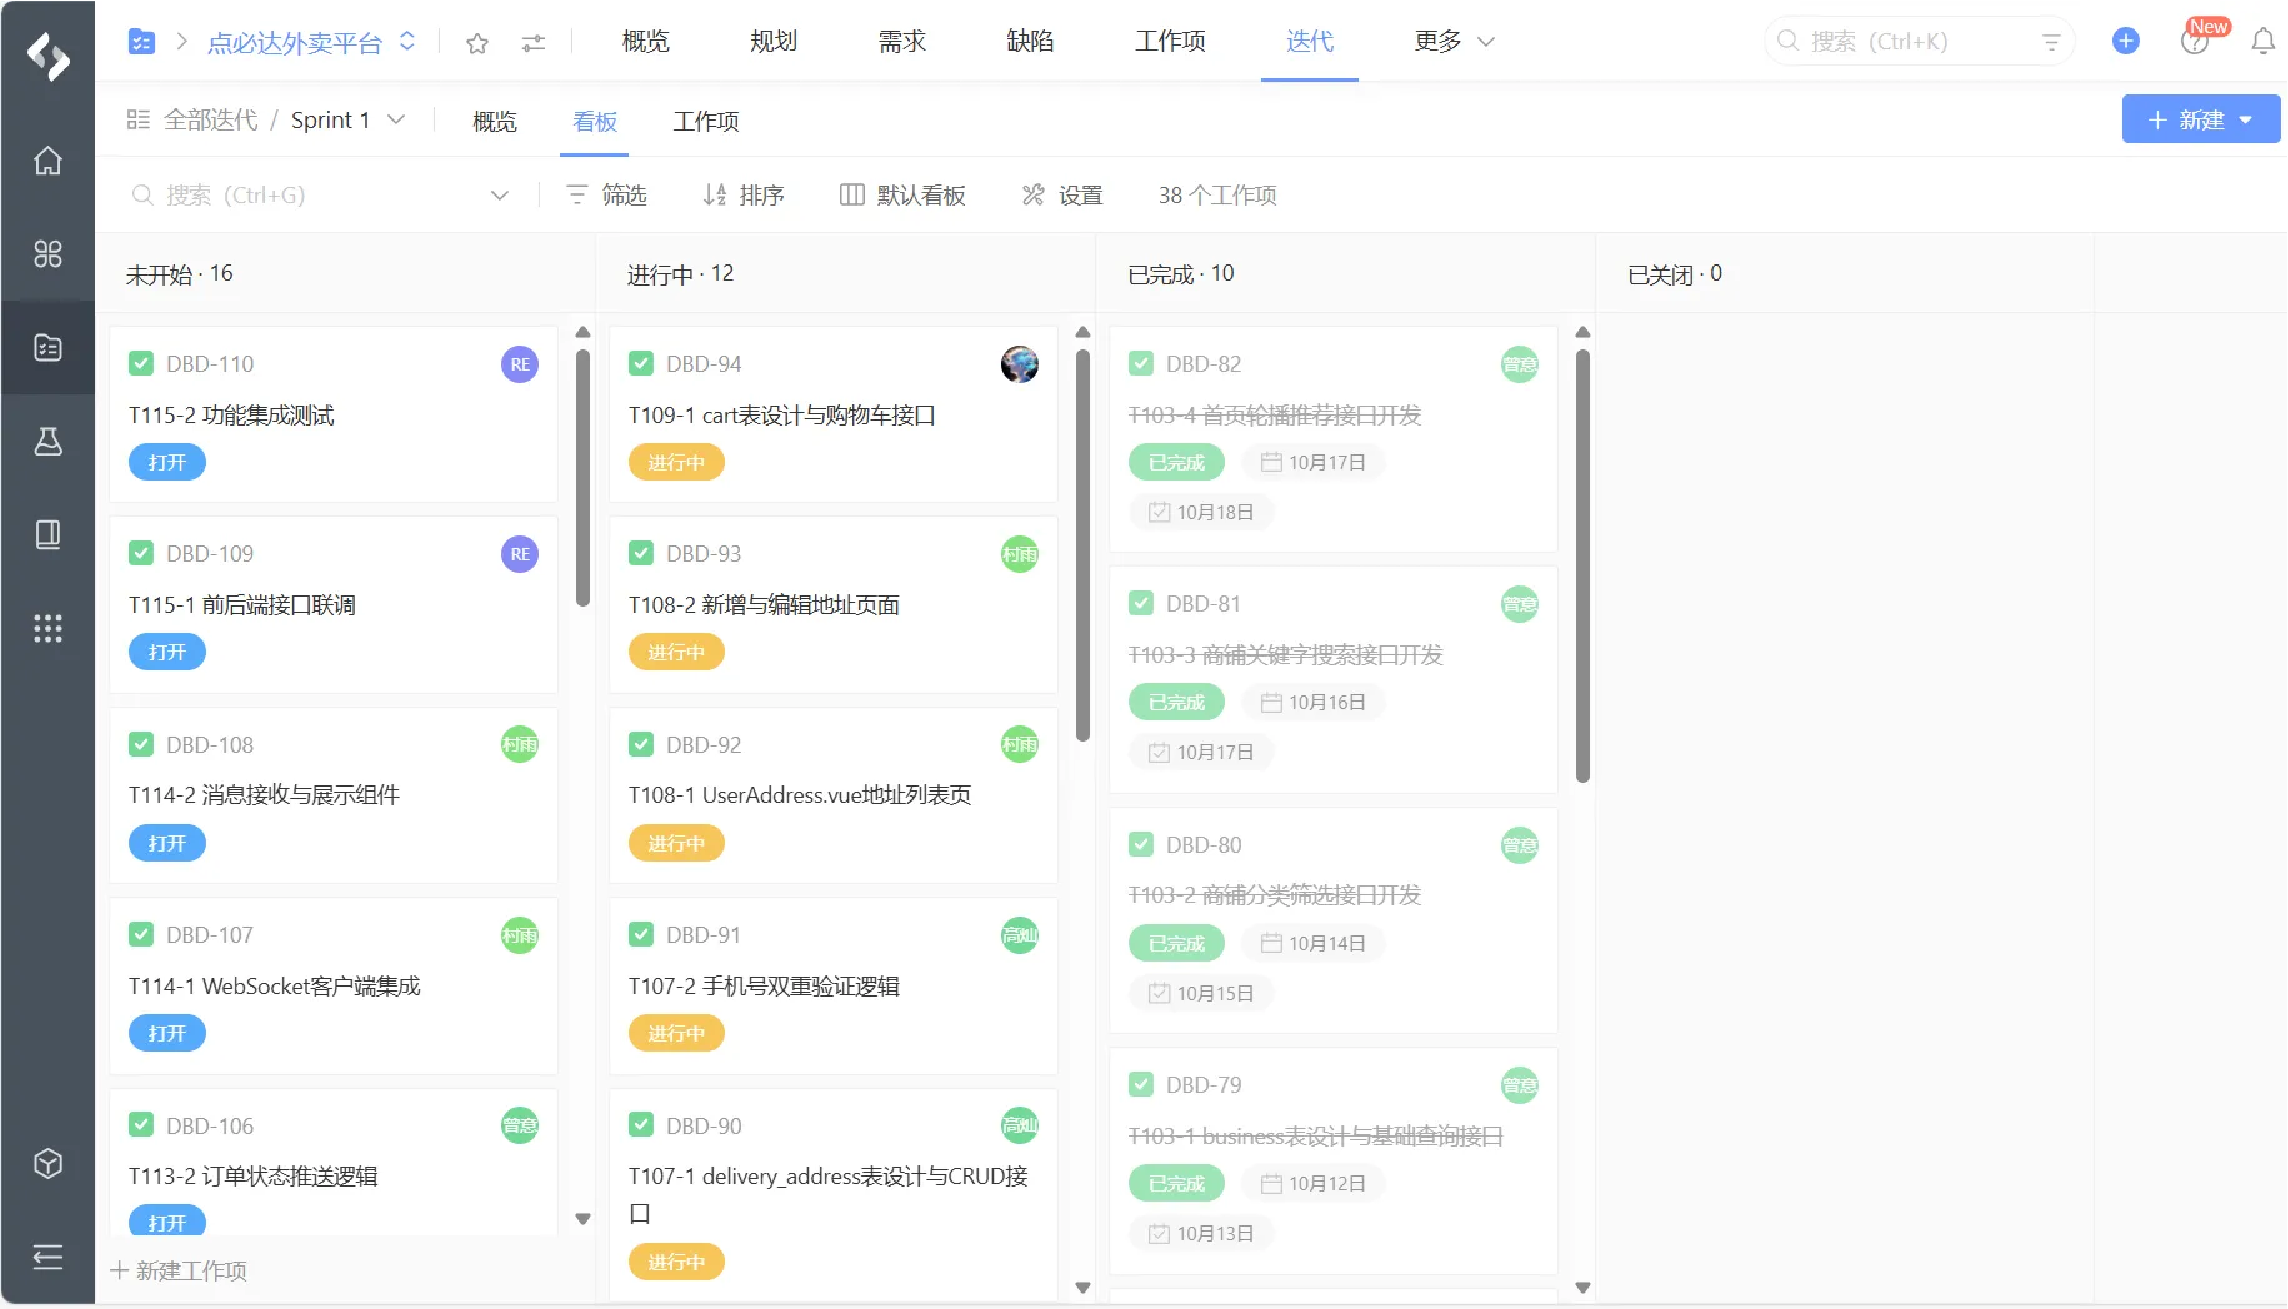
\includegraphics[width=1\textwidth]{figures/in/image1}
                  \caption{Sprint1燃尽图数据来源}
              \end{figure}

        \item \textbf{燃尽图图表}
              \begin{figure}[H]
                  \centering
                  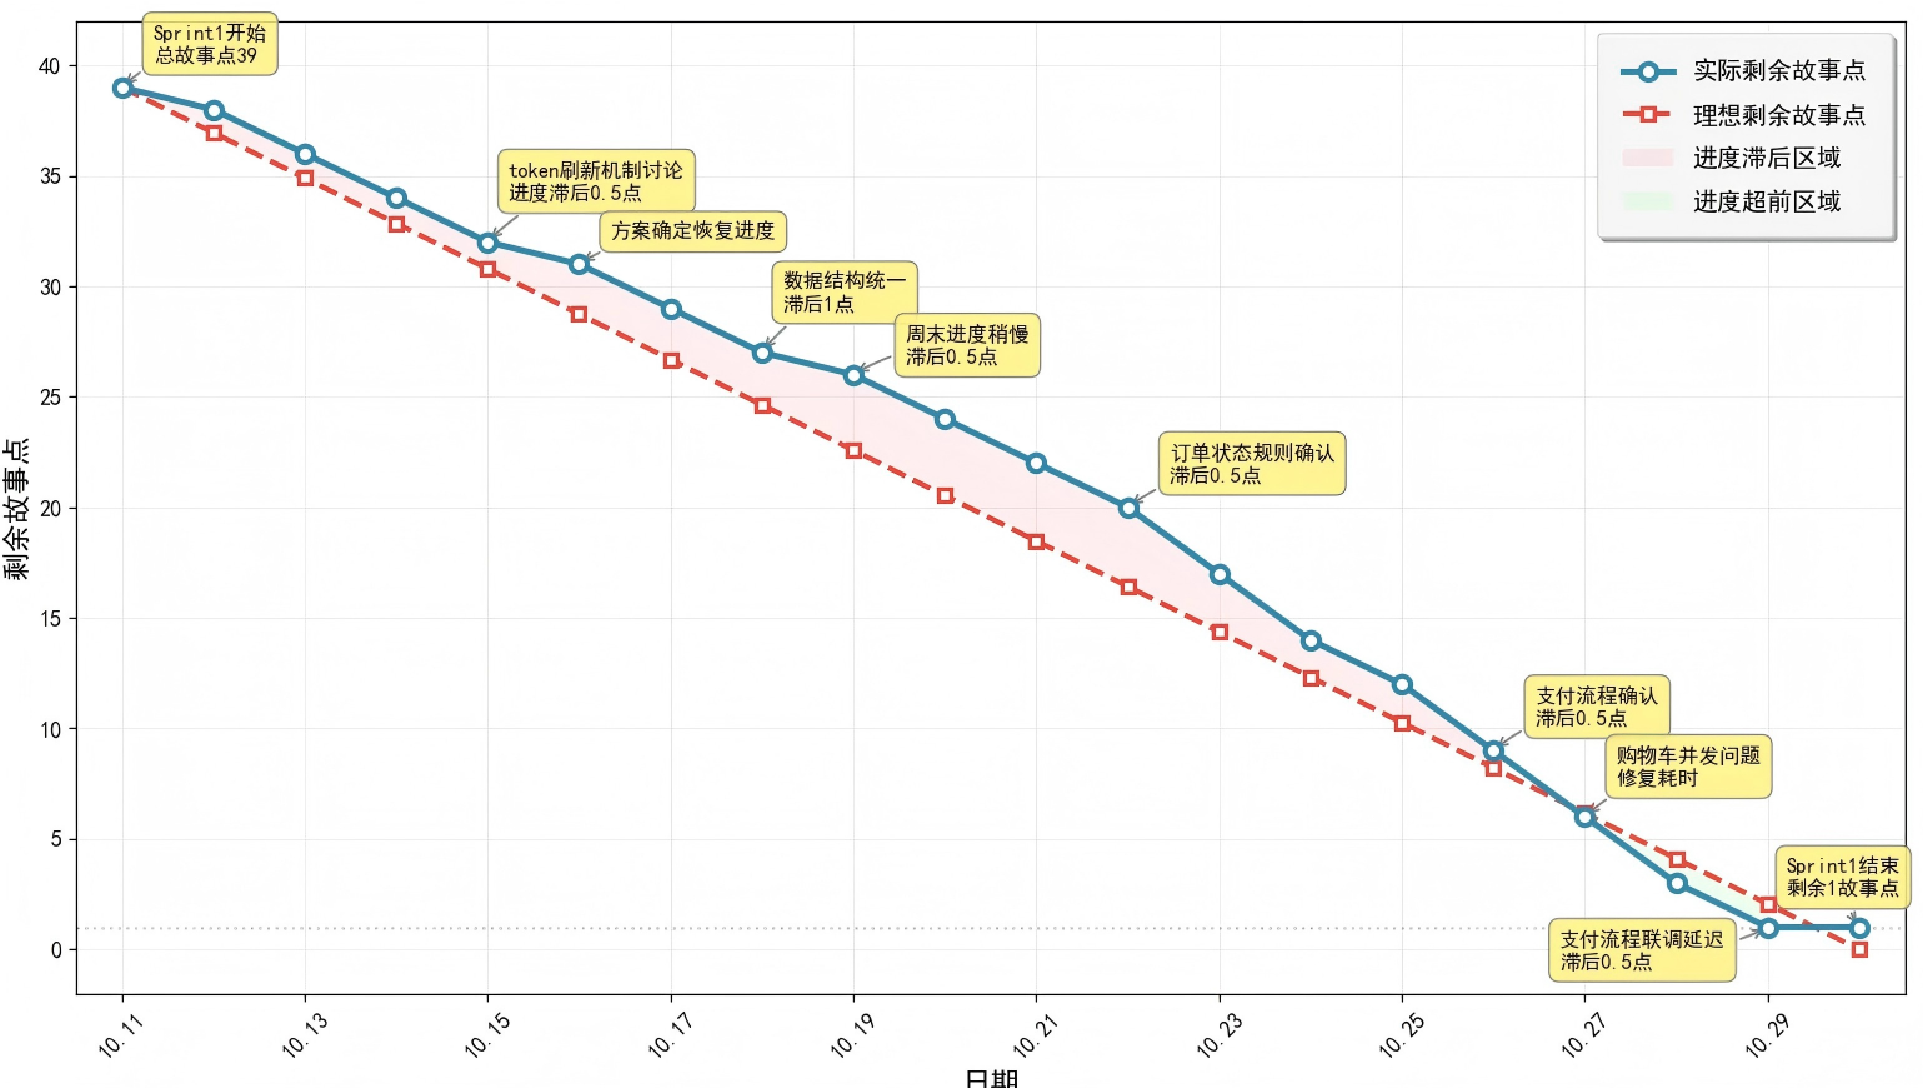
\includegraphics[width=1\textwidth]{figures/in/fire1}
                  \caption{Sprint1燃尽图 (10.11-10.30)}
              \end{figure}


        \item \textbf{进度偏差分析}
              \begin{itemize}
                  \item 偏差点 1（10.15）
                        \begin{itemize}
                            \item 偏差情况：因token刷新机制技术方案讨论，T101-3 Spring Security配置延误1小时。
                            \item 影响分析：用户认证模块进度滞后，可能影响前端路由守卫开发。
                            \item 解决方案：Scrum Master高灿组织戴茗静和曾意进行技术方案讨论，确定采用refresh token方案。
                            \item 偏差量：约0.5个故事点
                        \end{itemize}

                  \item 偏差点 2（10.18）
                        \begin{itemize}
                            \item 偏差情况：购物车数据结构和轮播数据格式需要统一确认，多个任务进度受阻。
                            \item 影响分析：购物车接口开发和商铺详情页开发均受到影响。
                            \item 解决方案：戴茗静与贾思韵会后确认数据结构，统一前后端数据格式。
                            \item 偏差量：约1个故事点
                        \end{itemize}

                  \item 偏差点3（10.19）
                        \begin{itemize}
                            \item 偏差情况：周末开发进度放缓，团队参与度不高。
                            \item 影响分析：整体进度有所滞后，需工作日追赶。
                            \item 解决方案：Scrum Master提醒团队合理安排周末工作时间。
                            \item 偏差量：约0.5个故事点
                        \end{itemize}

                  \item 偏差点4（10.22）
                        \begin{itemize}
                            \item 偏差情况：订单状态流转规则需要确认，订单创建功能开发受阻。
                            \item 影响分析：订单模块核心功能开发进度滞后。
                            \item 解决方案：戴茗静与贾思韵确定状态机规则，明确状态流转逻辑。
                            \item 偏差量：约0.5个故事点
                        \end{itemize}

                  \item 偏差点 5（10.25）
                        \begin{itemize}
                            \item 偏差情况：支付流程细节需要确认，支付页面开发受阻。
                            \item 影响分析：支付功能联调时间可能被压缩。
                            \item 解决方案：贾思韵与戴茗静确定支付流程细节，包括地址选择、支付方式、成功跳转等。
                            \item 偏差量：约0.5个故事点
                        \end{itemize}

                  \item 偏差点 6（10.27）
                        \begin{itemize}
                            \item 偏差情况：测试发现购物车并发问题，需要修复。
                            \item 影响分析：修复bug占用开发时间，影响测试进度。
                            \item 解决方案：戴茗静优化购物车锁机制，确保并发安全。
                            \item 偏差量：约1个故事点
                        \end{itemize}
                  \item 偏差点 7（10.29）
                        \begin{itemize}
                            \item 偏差情况：支付接口联调时，跳转页面参数传递异常。
                            \item 影响分析：跳转界面进度滞后，影响测试进度。
                            \item 解决方案：戴茗静与杨晓越协同排查，修复后因时间紧张，仅完成基础跳转，未实现订单详情自动加载。
                            \item 偏差量：约0.5个故事点。
                        \end{itemize}

              \end{itemize}

    \end{enumerate}
    \textbf{偏差总结：} Sprint1 计划完成 39 个故事点，实际完成 38 个故事点，因支付流程联调延迟与购物车并发问题修复，累计偏差 1 个故事点。核心 MVP 功能（用户注册登录、商铺查询下单、订单推送）均已交付，仅 “支付成功后自动跳转至订单详情” 功能延迟至 Sprint2 优化，整体满足最小可用版本标准。

\end{levellist}


\subsection{Sprint2:商家管理核心功能 + 用户互动体验升级(10.31-11.16)}

\begin{levellist}
    \item \textbf{Sprint 规划会记录}
    \begin{itemize}
        \item 会议时间：2025年10月31日 19:00-20:30
        \item 参会人员：全体成员（Product Owner贾思韵主导，前后端共同估算工时）
        \item Sprint 目标：建立商家入驻和运营管理能力，实现商家从开店到接单的完整工作流，同时增强用户互动功能。
        \item Sprint Backlog（前后端任务整合，关联用户故事）：

              \begin{longtable}{>{\centering\arraybackslash}m{1.4cm} >{\centering\arraybackslash}m{3.1cm} >{\centering\arraybackslash}m{1.7cm} >{\centering\arraybackslash}m{1.8cm} >{\centering\arraybackslash}m{1.8cm} >{\centering\arraybackslash}m{1.3cm} >{\centering\arraybackslash}m{1.2cm}}

                  \caption{Sprint2前后端任务整合与关联用户故事} \label{tab:training}                                                                                                                    \\

                  \toprule
                  \textbf{任务ID} & \textbf{任务名称}                                                  & \textbf{关联用户故事} & \textbf{负责成员} & \textbf{预估工时(小时)} & \textbf{依赖关系}    & \textbf{任务状态} \\
                  \midrule
                  \endfirsthead

                  \multicolumn{7}{c}{{\tablename\ \thetable{} 续表}}                                                                                                                        \\
                  \toprule
                  \textbf{任务ID} & \textbf{任务名称}                                                  & \textbf{关联用户故事} & \textbf{负责成员} & \textbf{预估工时(小时)} & \textbf{依赖关系}    & \textbf{任务状态} \\
                  \midrule
                  \endhead

                  \bottomrule
                  \endfoot


                  T201-1        & 商家入驻申请提交与数据模型接口开发                                              & US006           & 戴茗静           & 3                 & 无                & 待办            \\
                  T201-2        & 商家申请列表与详情查询接口开发                                                & US006           & 戴茗静           & 2                 & 依赖T201-1         & 待办            \\
                  T202-1        & ApplyMerchant.vue申请表单页面开发                                      & US006           & 杨晓越           & 3                 & 无                & 待办            \\
                  T202-2        & 资质文件上传组件集成与预览                                                  & US006           & 杨晓越           & 2                 & 无                & 待办            \\
                  T202-3        & 申请提交与状态提示功能                                                    & US006           & 杨晓越           & 1                 & 依赖T201-1, T202-1 & 待办            \\
                  T203-1        & 商品CRUD（增删改查）接口开发                                               & US008           & 高灿            & 3                 & 依赖店铺权限校验         & 待办            \\
                  T203-2        & 商品上架/下架状态接口开发                                                  & US008           & 高灿            & 2                 & 依赖T203-1         & 待办            \\
                  T203-3        & 权限校验中间件（商家本人操作）                                                & US008           & 高灿            & 2                 & 无                & 待办            \\
                  T204-1        & MerchantFood.vue商品列表页开发                                        & US008           & 贾思韵           & 3                 & 依赖T203-1         & 待办            \\
                  T204-2        & 商品新增/编辑弹窗表单组件                                                  & US008           & 贾思韵           & 3                 & 依赖T204-1         & 待办            \\
                  T205-1        & 收藏/点赞统一互动接口开发                                                  & US011           & 曾意            & 3                 & 依赖商铺、用户表         & 待办            \\
                  T205-2        & 用户收藏列表查询接口开发                                                   & US011           & 曾意            & 2                 & 依赖T205-1         & 待办            \\
                  T205-3        & 商铺互动数据（点赞/收藏数）聚合查询接口                                           & US011           & 曾意            & 3                 & 依赖T205-1         & 待办            \\
                  T206-1        & BusinessInfo.vue收藏点赞按钮组件                                       & US011           & 杨晓越           & 2                 & 依赖T205-1         & 待办            \\
                  T206-2        & Favorites.vue我的收藏页面开发                                          & US011           & 杨晓越           & 3                 & 依赖T205-2         & 待办            \\
                  T206-3        & 互动状态初始化与持久化逻辑                                                  & US011           & 杨晓越           & 2                 & 依赖T206-1         & 待办            \\
                  T207-1        & 商铺互动数据（点赞/收藏数）聚合接口开发                                           & US017           & 曾意            & 3                 & 依赖T205-1         & 待办            \\
                  T207-2        & 综合评分计算逻辑实现                                                     & US017           & 曾意            & 2                 & 依赖T207-1         & 待办            \\
                  T207-3        & 多商铺数据汇总与缓存优化                                                   & US017           & 曾意            & 3                 & 依赖T207-2         & 待办            \\
                  T208-1        & MerchantStats.vue人气统计页面开发                                      & US017           & 杨晓越           & 2                 & 依赖T207-1         & 待办            \\
                  T208-2        & 人气数据排序与可视化展示功能                                                 & US017           & 杨晓越           & 2                 & 依赖T208-1         & 待办            \\
                  T209-1        & 商家端完整流程联调（申请->商品管理）                                            & -               & 任晓华           & 1                 & 依赖所有开发任务         & 待办            \\
                  T209-2        & 用户互动功能端到端测试                                                    & US011           & 任晓华           & 4                 & 依赖T205, T206系列   & 待办            \\
                  T209-3        & Bug修复与代码审查，同时修复Sprint1中的“支付成功后自动跳转至订单详情”功能问题，完成Sprint1遗留的1个故事点 & -               & 戴茗静/曾意        & 4                 & 依赖T209-1, T209-2 & 待办            \\
                  T209-4        & Sprint2 预生产环境部署与冒烟测试                                           & -               & 曾意            & 4                 & 依赖T209-3         & 待办            \\
              \end{longtable}


        \item 总工时与里程碑：
              \begin{itemize}
                  \item 总工时：64小时（前端24小时，后端30小时，测试与部署10小时）
                  \item 关键里程碑：
                        \begin{enumerate}
                            \item 11月3日前：完成后端商家入驻申请与收藏点赞基础接口，前端完成申请页面与互动按钮组件。
                            \item 11月8日前：完成后端商品管理与商家统计接口，前端完成商品管理页面与收藏列表页。
                            \item 11月12日前：完成商家核心功能（入驻、商品管理）的前后端联调，完成商家人气统计模块开发。
                            \item 11月15日前：完成所有功能集成测试、Bug修复及预生产环境部署。
                            \item 11月16日：Sprint2结束，核心功能（商家入驻、商品管理、收藏点赞）全部落地，仅“商家统计数据实时同步”功能部分完成（延迟至Sprint3优化），累计偏差0.5个故事点
                        \end{enumerate}

              \end{itemize}

    \end{itemize}

    \item \textbf{每日站会记录}

    \begin{longtable}{>{\centering\arraybackslash}m{1cm} >{\centering\arraybackslash}m{1cm} >{\centering\arraybackslash}m{9cm} >{\centering\arraybackslash}m{2.5cm}}

        \caption{Sprint2每日站会记录} \label{tab:training}                                                                                                                                                                  \\

        \toprule
        \textbf{日期}                                             & \textbf{参会人员}                                          & \textbf{核心内容}                                                             & \textbf{阻碍与解决} \\
        \midrule
        \endfirsthead

        \multicolumn{4}{c}{{\tablename\ \thetable{} 续表}}                                                                                                                                                              \\
        \toprule
        \textbf{日期}                                             & \textbf{参会人员}                                          & \textbf{核心内容}                                                             & \textbf{阻碍与解决} \\
        \midrule
        \endhead

        \bottomrule
        \endfoot


        10月31日                                                  & 全体                                                     & - 贾思韵： 昨天完成Sprint1回顾会；今天主持Sprint2规划会，明确Sprint目标为“建立商家入驻和运营管理能力”。 \newline
        - 戴茗静：今天分析US006（成为商家）接口需求，准备开始T201-1。 \newline
        - 全体： 确认Sprint2包含US006、US008、US011、US017，共4个用户故事。       & 状态：Sprint2正式启动                                                                                                                                      \\
        11月1日                                                   & 全体                                                     & - 戴茗静： 昨天完成T201-1商家入驻申请接口的数据模型设计；今天开始编写提交接口逻辑。 \newline
        - 曾意： 昨天分析US011和US017；今天设计merchant\_interaction表结构，准备T205-1。 \newline
        - 杨晓越： 昨天熟悉商家端组件库；今天开始搭建ApplyMerchant.vue（T202-1）页面框架。  & 无阻碍 - 整体进入设计与开发启动阶段。                                                                                                                                \\
        11月2日                                                   & 全体                                                     & - 戴茗静： 昨天完成T201-1接口主体开发；今天进行单元测试和文档编写。 \newline
        - 杨晓越： 昨天完成T202-1页面基础布局；今天细化表单字段UI和样式。 \newline
        - 高灿： 昨天分析US008商品管理业务逻辑；今天开始设计商品表增删改查接口（T203-1）。        & 无阻碍 - 各任务按计划推进。                                                                                                                                     \\
        11月3日                                                   & 全体                                                     & - 戴茗静： 昨天完成T201-1；今天开始开发T201-2（申请列表查询接口）。 \newline
        - 杨晓越： 昨天完成T202-1样式优化；今天开始开发T202-2（资质文件上传组件）。\newline
        - 高灿： 昨天完成T203-1商品查询接口；今天开发商品新增和修改接口。 \newline
        - 曾意： 昨天完成数据库设计；今天开始开发T205-1收藏/点赞统一接口。                  & 进度： 第一个接口T201-1完成，首个用户故事(US006)后端部分取得进展。                                                                                                            \\
        11月4日                                                   & 全体                                                     & - 杨晓越： 昨天完成T202-2文件上传组件基础功能；今天集成OSS SDK并优化上传体验。 \newline
        - 高灿： 昨天完成商品增改接口；今天开发商品删除与状态（上架/下架）接口（T203-2）。 \newline
        - 曾意： 昨天完成T205-1接口基础逻辑；今天完善添加/取消收藏点赞的状态切换与数据一致性。 \newline
        - 贾思韵： 昨天分析商品管理页面需求；今天开始设计MerchantFood.vue（T204-1）页面结构。 & 无阻碍 - 核心接口与组件并行开发中。                                                                                                                                 \\
        11月5日                                                   & 全体                                                     & - 戴茗静： 昨天完成T201-2；今天等待前端联调。、 \newline
        - 杨晓越： 昨天完成T202-2与OSS集成；今天开发T202-3（申请提交与状态提示），并与后端T201-1联调。 \newline
        - 高灿： 昨天完成T203-2；今天开发T203-3（权限校验中间件），确保仅商家本人可操作商品。 \newline
        - 曾意： 昨天完成T205-1接口测试；今天开始开发T205-2（用户收藏列表查询接口）。          & 进度： US006（成为商家）前后端功能进入联调阶段，完成约2个故事点。                                                                                                                \\
        11月6日                                                   & 全体                                                     & - 杨晓越： 昨天完成T202-3联调，申请流程基本跑通；今天开始开发T206-1（商铺详情页收藏点赞按钮）。 \newline
        - 高灿： 昨天完成T203-3；今天对商品管理所有接口（T203系列）进行集成测试。 \newline
        - 贾思韵： 昨天完成T204-1页面结构设计；今天开始编码，实现商品列表渲染。 \newline
        - 曾意： 昨天完成T205-2；今天开始设计T205-3（商铺互动数据聚合接口）。              & 阻碍： T206-1前端开发依赖T205-1接口提供。 \newline
        解决： 曾意确认T205-1接口已就绪，杨晓越可调用。                                                                                                                                                                                   \\
        11月7日                                                   & 全体                                                     & - 贾思韵： 昨天完成T204-1商品列表展示；今天开发商品操作栏（上架/下架/编辑按钮）。 \newline
        - 杨晓越： 昨天完成T206-1按钮组件基础交互；今天开发点击事件并与T205-1接口联调。 \newline
        - 曾意： 昨天完成T205-3接口设计；今天开发数据聚合逻辑，计算商铺的点赞、收藏总数。 \newline
        - 任晓华： 昨天开始编写测试用例；今天对已完成的申请流程（US006）进行功能测试。             & 进度： US011（收藏点赞）核心交互功能开发完成，进入联调。                                                                                                                     \\
        11月8日                                                   & 全体                                                     & - 贾思韵： 昨天完成T204-1操作功能；今天开始开发T204-2（商品新增/编辑弹窗表单）。 \newline
        - 杨晓越： 昨天完成T206-1联调；今天开始开发T206-2（我的收藏页面）。 \newline
        - 曾意： 昨天完成T205-3；今天根据US017需求，开始设计商家人气统计接口（T207-1）。 \newline
        - 高灿： 昨天完成接口测试；今天协助贾思韵进行T204-1与T203系列接口的联调。             & 无阻碍 - 开发重心向商家运营功能（商品管理、统计）转移。                                                                                                                       \\
        11月9日                                                   & 全体                                                     & - 贾思韵： 昨天完成T204-2弹窗表单基础功能；今天实现表单数据回填（编辑时）和提交逻辑。 \newline
        - 杨晓越： 昨天完成T206-2收藏列表页面布局；今天实现列表数据渲染，并与T205-2接口联调。 \newline
        - 曾意： 昨天完成T207-1接口设计，确定统计维度为点赞数、收藏数；今天开始开发商铺互动数据聚合接口。 \newline
        - 任晓华： 昨天测试申请功能；今天开始测试商品管理流程（US008）。                    & 阻碍： T204-2编辑回填时，商品图片处理逻辑需明确。 \newline
        解决： 高灿确认沿用T203-1的图片字段处理方式，无需额外接口。                                                                                                                                                                             \\
        11月10日                                                  & 全体                                                     & - 贾思韵： 昨天完成T204-2与后端联调；今天整体优化MerchantFood.vue页面交互体验。 \newline
        - 杨晓越： 昨天完成T206-2联调；今天开发T206-3（互动状态初始化与持久化），确保用户登录后按钮状态正确。 \newline
        - 曾意： 昨天完成T207-1基础数据聚合；今天开发T207-2（综合评分计算逻辑）。 \newline
        - 戴茗静： 昨天支持其他任务；今天开始为下周的集成测试做准备。                        & 进度： US008（商品管理）核心功能开发与联调完成，完成约5个故事点。                                                                                                                \\
        11月13日                                                  & 全体                                                     & - 杨晓越： 昨天完成T206-3；今天开始开发MerchantStats.vue人气统计页面（T208-1）。 \newline
        - 曾意： 昨天完成T207-2综合评分算法；今天开发T207-3（多商铺数据汇总与缓存优化）。 \newline
        - 贾思韵： 昨天优化商品管理页；今天协助杨晓越设计仪表盘的数据展示样式。 \newline
        - 任晓华： 昨天完成商品管理功能测试；今天开始对收藏点赞功能（US011）进行端到端测试（T209-2）。  & 阻碍：T208-1前端开发依赖T207系列接口数据格式，且统计数据实时同步逻辑需额外联调。 \newline
        解决：曾意提供响应示例文档，前后端对齐数据格式，但实时同步逻辑需简化实现，完整功能延迟至Sprint3                                                                                                                                                           \\
        11月14日                                                  & 全体                                                     & - 杨晓越： 昨天完成T208-1页面基础框架；今天开发人气数据排序与可视化展示功能（T208-2）。 \newline
        - 曾意： 昨天完成T207-3；今天配合杨晓越调试MerchantStats.vue页面的数据对接。 \newline
        - 任晓华： 昨天在US011测试中发现取消收藏后列表未实时更新的问题；今天与杨晓越、曾意定位问题。 \newline
        - 全体： 下午计划开始Sprint2的全面集成联调（T209-1）。                     & 阻碍： 收藏列表实时更新存在延迟。 \newline
        解决： 确认为前端状态管理问题，杨晓越修复后由任晓华复测。                                                                                                                                                                                 \\
        11月15日                                                  & 全体                                                     & - 全体： 昨天启动集成联调（T209-1），重点验证商家从申请->登录->商品管理->查看统计的完整流程。 \newline
        - 任晓华： 主导联调，联调发现3个问题：1)申请后状态提示不明显；2)商品下架后在前台仍有缓存；3)商家统计数据实时同步存在2秒延迟（简化为5秒同步，完整优化延迟）。 \newline
        - 戴茗静/曾意： 负责T209-3（Bug修复），分别处理后端相关问题，完成Sprint1遗留的1个故事点。 \newline
        - 杨晓越/贾思韵： 负责修复前端相关问题（提示、页面样式）。                         & 状态： 进入集中修复阶段。问题已明确，分配至具体负责人。                                                                                                                        \\
        11月16日                                                  & 全体                                                     & - 全体： 昨天完成所有关键Bug的修复和验证。 \newline
        - 曾意： 昨天完成T209-4，将修复后的代码部署至预生产环境，并进行冒烟测试通过。 \newline
        - 任晓华： 验收测试通过，核心工作流（US006、US008、US011、US017）全部通畅，仅“商家统计数据实时同步（误差≤2秒）”未完全达标（当前误差5秒），纳入Sprint3优化。\newline
        - 贾思韵： 整理Sprint2演示内容。                                   & 状态：Sprint2核心目标达成，仅部分功能未达标，累计偏差0.5个故事点。                                                                                                              \\
    \end{longtable}

    \item \textbf{Sprint 评审会记录}
    \begin{itemize}
        \item 会议时间：2025年11月16日 15:00-16:30
        \item 验收人员：Product Owner贾思韵 + 全体成员
        \item 验收结果（按用户故事）：
              \begin{enumerate}
                  \item US006（成为商家）：验收通过 \\
                        满足“顾客提交商家申请”、“商家填写商铺信息提交申请”、“申请后进入‘审核中’状态”等核心验收标准。前后端流程完整，演示顺利。
                  \item US008（商品管理）：验收通过 \\
                        满足“商家可查看本店商品列表”、“可执行上架/下架操作”、“可修改商品信息（名称、价格、图片等）”、“可删除商品”及“操作权限校验正确”等所有验收标准。商品管理核心工作流稳定可用。
                  \item US011（收藏点赞）：验收通过 \\
                        满足“商铺详情页点赞/收藏按钮即时交互”、“‘我的收藏’列表正确展示”、“点赞数/收藏数在商家端与用户端实时同步”等验收标准。用户互动功能完整，体验流畅。
                  \item US017（商家人气统计）：部分通过 \\
                        满足“展示点赞数、收藏数、综合评分”核心标准，但“统计数据实时
              \end{enumerate}
              同步（误差≤2秒）”未达标（当前误差5秒），需Sprint3优化，按0.5个故事点部分完成计算。
    \end{itemize}

    \item \textbf{Sprint 回顾会记录}
    \begin{itemize}
        \item 会议时间：2025年11月16日 17:00-18:00
        \item 讨论内容（3个核心问题）：\\
              \textbf{做得好的地方}
              \begin{enumerate}
                  \item 接口文档评审环节有效，前后端理解一致性问题大幅减少。
                  \item 商家端功能模块划分清晰，开发效率较高。
                  \item 性能测试checklist得到应用，核心接口响应时间达标。
              \end{enumerate}
              \textbf{需要改进的地方}
              \begin{enumerate}
                  \item 商家业务流程测试覆盖不够全面；复杂功能（如实时数据同步）的联调时间预估不足；非核心功能的优先级排序需更明确。
                  \item 部分复杂前端交互开发时间估算仍偏乐观。
                  \item 数据统计功能的业务依赖关系前期分析不足。
              \end{enumerate}
              \textbf{下一轮改进措施}
              \begin{enumerate}
                  \item 增加业务流程的端到端测试用例，覆盖异常场景。
                  \item 复杂交互任务强制进行技术方案评审后再开始开发。
                  \item 功能规划时明确外部依赖和前置条件，避免开发阻塞。
              \end{enumerate}
    \end{itemize}

    \item \textbf{Sprint 进度可视化（燃尽图）}
    \begin{enumerate}
        \item \textbf{燃尽图基础信息}
              \begin{itemize}
                  \item 迭代周期：2025年10月31日 - 11月16日
                  \item 跟踪对象：Sprint2 Backlog中的4个用户故事（US006、US008、US011、US017）
                  \item 总故事点：14点
                  \item 数据来源：PingCode 看板每日更新的任务状态
              \end{itemize}

              \begin{figure}[H]
                  \centering
                  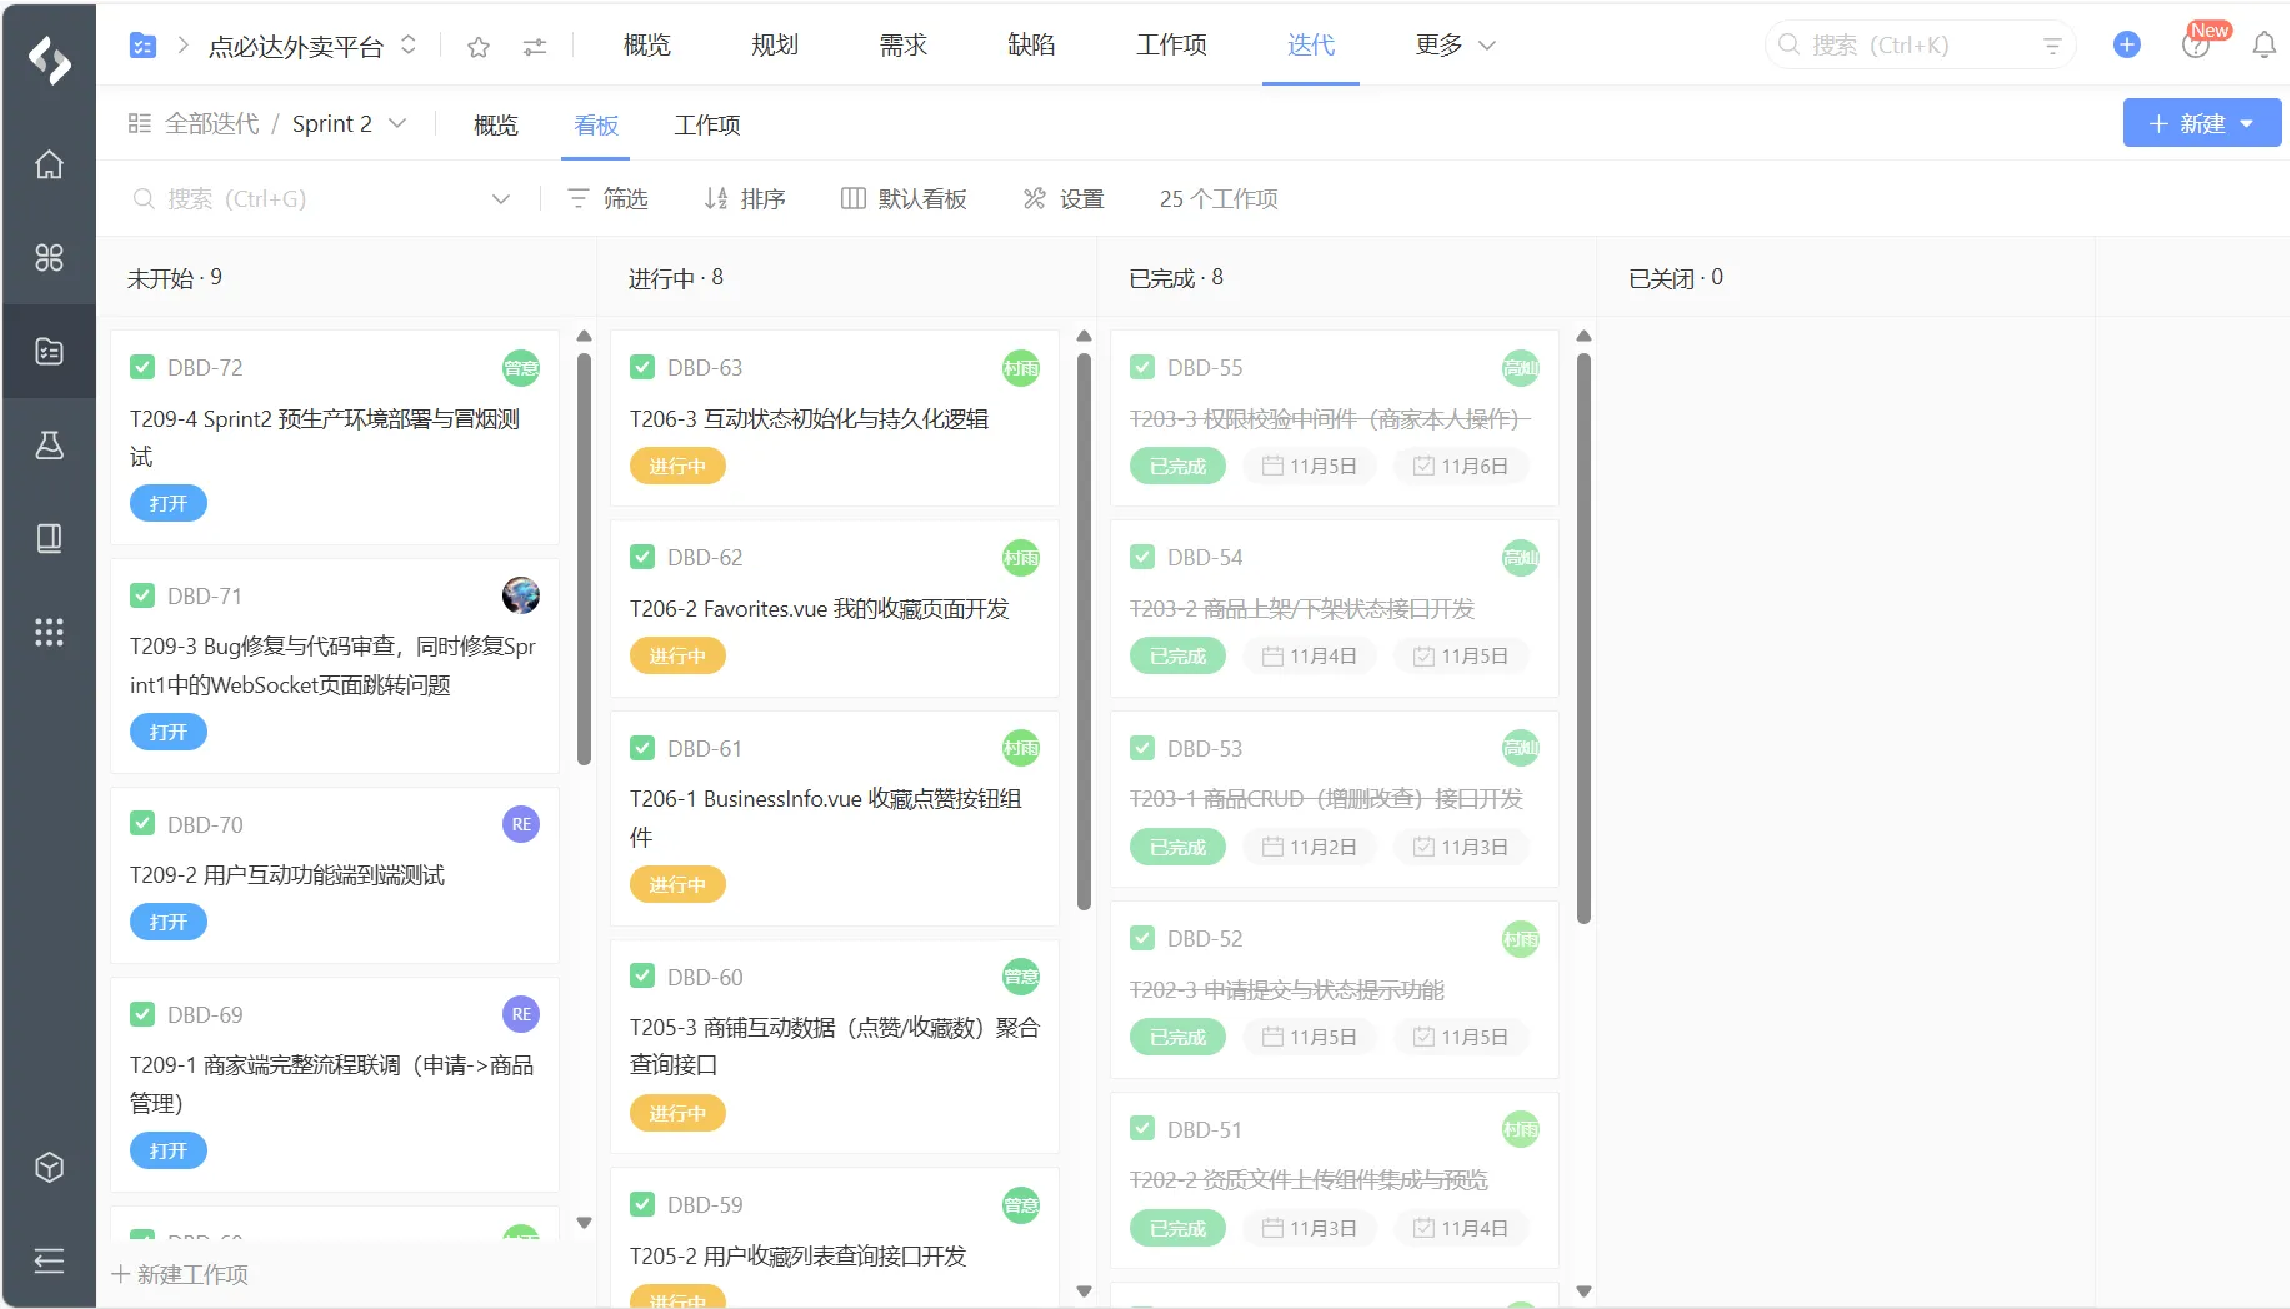
\includegraphics[width=1\textwidth]{figures/in/image2}
                  \caption{Sprint2燃尽图数据来源}
              \end{figure}


        \item \textbf{燃尽图图表}
              \begin{figure}[H]
                  \centering
                  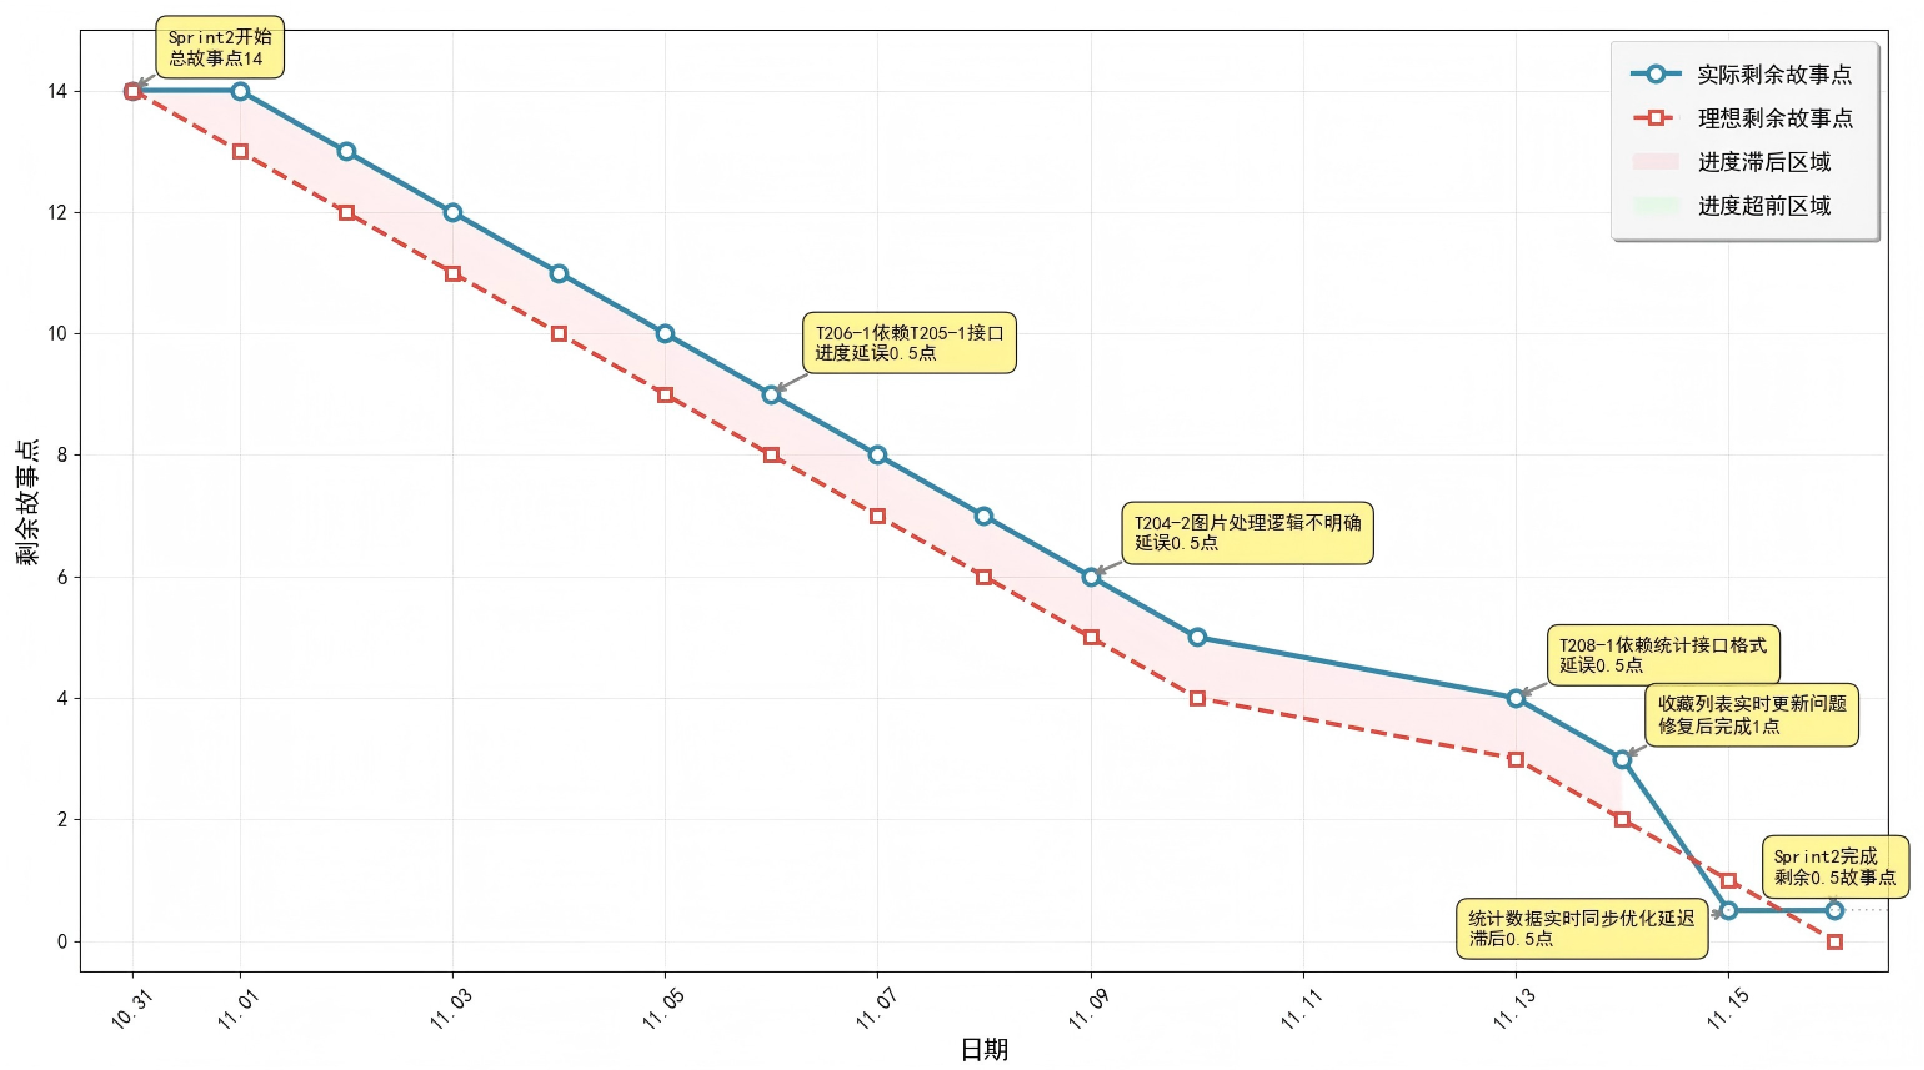
\includegraphics[width=1\textwidth]{figures/in/fire2}
                  \caption{Sprint2燃尽图 (10.31-11.16)}
              \end{figure}

        \item \textbf{进度偏差分析}
              \begin{itemize}
                  \item 偏差点 1（11.06）
                        \begin{itemize}
                            \item 偏差情况：T206-1（商铺详情页收藏点赞按钮）前端开发依赖T205-1（收藏/点赞统一接口），接口就绪状态确认延迟导致开发受阻。
                            \item 影响分析：US011（收藏点赞）前端交互功能开发滞后，可能影响后续联调计划。
                            \item 解决方案：Scrum Master组织曾意与杨晓越同步接口状态，曾意确认T205-1接口已就绪并提供调用文档，杨晓越立即启动开发。
                            \item 偏差量：约0.5个故事点
                        \end{itemize}

                  \item 偏差点 2（11.09）
                        \begin{itemize}
                            \item 偏差情况：T204-2（商品新增/编辑弹窗表单）开发中，商品图片处理逻辑与后端接口规范未明确，导致数据回填功能开发暂停。
                            \item 影响分析：US008（商品管理）编辑功能联调进度滞后，可能压缩后续测试时间。
                            \item 解决方案：高灿与贾思韵快速对齐技术方案，确认沿用T203-1（商品查询接口）的图片字段处理方式，无需新增接口。
                            \item 偏差量：约0.5个故事点
                        \end{itemize}

                  \item 偏差点3（11.13）
                        \begin{itemize}
                            \item 偏差情况：T208-1页面开发依赖T207系列接口返回的人气数据格式，前后端格式未提前对齐导致开发阻塞。
                            \item 影响分析：US017（商家人气数据统计）前端可视化开发受阻，人气数据展示功能进度滞后。
                            \item 解决方案：曾意紧急提供T207系列接口响应示例文档，杨晓越与曾意现场对齐字段定义和数据结构。
                            \item 偏差量：约0.5个故事点
                        \end{itemize}

                  \item 偏差点4（（11.14）
                        \begin{itemize}
                            \item 偏差情况：US011（收藏点赞）端到端测试中发现取消收藏后列表未实时更新，定位为前端Vuex状态管理未同步问题。
                            \item 影响分析：收藏功能用户体验不符合预期，验收测试不通过，需占用开发时间修复。
                            \item 解决方案：杨晓越优先修复状态管理逻辑，在取消收藏接口回调中强制刷新列表数据，任晓华同步完成复测。
                            \item 偏差量：约0.5个故事点
                        \end{itemize}

                  \item 偏差点 5（11.15）
                        \begin{itemize}
                            \item 偏差情况：商家统计数据实时同步逻辑复杂，联调时间不足，简化为 5 秒同步。
                            \item 影响分析：完整优化延迟至 Sprint3。
                            \item 解决方案：曾意编写临时同步方案，确保数据准确性，Sprint3 补充实时性优化。
                            \item 偏差量：约0.5个故事点
                        \end{itemize}

              \end{itemize}

    \end{enumerate}
    \textbf{偏差总结：} Sprint2 计划完成 14 个故事点，实际完成 13.5 个故事点，因技术依赖不明确、接口规范未对齐、状态管理缺陷及实时同步复杂度高，累计偏差 0.5 个故事点。核心商家端功能（商家入驻申请、商品管理、收藏点赞互动）均已高质量交付并通过验收，仅 "统计数据实时同步（误差≤2秒）" 功能未达验收标准（当前误差5秒），延迟至 Sprint3 优化。

\end{levellist}



\subsection{Sprint3:管理端完善 + 高级功能扩展 + 系统优化(11.17-12.7)}

\begin{levellist}
    \item \textbf{Sprint 规划会记录}
    \begin{itemize}
        \item 会议时间： 2025年11月17日 19:00-20:30
        \item 参会人员： 全体成员（Product Owner贾思韵主导，前后端共同估算工时）
        \item Sprint 目标： 建立管理端后台治理体系，完善平台审核与用户管理能力；集成AI智能客服与数据看板，提升系统整体安全性与运营支撑水平。
        \item Sprint Backlog（前后端任务整合，关联用户故事）：


              \begin{longtable}{>{\centering\arraybackslash}m{1.4cm} >{\centering\arraybackslash}m{3.1cm} >{\centering\arraybackslash}m{1.7cm} >{\centering\arraybackslash}m{1.8cm} >{\centering\arraybackslash}m{1.8cm} >{\centering\arraybackslash}m{1.3cm} >{\centering\arraybackslash}m{1.2cm}}

                  \caption{Sprint3前后端任务整合与关联用户故事} \label{tab:training}                                                                                                  \\

                  \toprule
                  \textbf{任务ID} & \textbf{任务名称}                & \textbf{关联用户故事}     & \textbf{负责成员} & \textbf{预估工时(小时)} & \textbf{依赖关系}                & \textbf{任务状态} \\
                  \midrule
                  \endfirsthead

                  \multicolumn{7}{c}{{\tablename\ \thetable{} 续表}}                                                                                                      \\
                  \toprule
                  \textbf{任务ID} & \textbf{任务名称}                & \textbf{关联用户故事}     & \textbf{负责成员} & \textbf{预估工时(小时)} & \textbf{依赖关系}                & \textbf{任务状态} \\
                  \midrule
                  \endhead

                  \bottomrule
                  \endfoot


                  T301-1        & 商家申请审核列表、详情与操作接口开发           & US009               & 高灿            & 5                 & 无                            & 待办            \\
                  T301-2        & 商铺申请审核列表、详情与操作接口开发           & US010               & 高灿            & 6                 & 无                            & 待办            \\
                  T302-1        & AdminAudit.vue商家/店铺审核页开发     & US009, US010        & 贾思韵           & 6                 & 依赖T301-2, T301-3             & 待办            \\
                  T302-2        & 审核操作交互、结果提交与状态反馈组件           & US009, US010        & 贾思韵           & 3                 & 依赖T302-1                     & 待办            \\
                  T303-1        & 用户管理（搜索、筛选、启用/禁用）接口开发        & US012               & 戴茗静           & 5                 & 无                            & 待办            \\
                  T303-2        & 商家集团与商铺管理（增删改查）接口开发          & US013               & 戴茗静           & 6                 & 无                            & 待办            \\
                  T304-1        & UserManagement.vue用户管理页面开发   & US012               & 杨晓越           & 5                 & 无                            & 待办            \\
                  T304-2        & AdminBusiness.vue商家与商铺管理页面开发 & US013               & 杨晓越           & 6                 & 依赖T303-2                     & 待办            \\
                  T305-1        & AI对话历史表设计与问答接口开发（集成DeepSeek） & US014               & 曾意            & 6                 & 无                            & 待办            \\
                  T305-2        & 审核结果通知（WebSocket）集成与推送逻辑优化   & US016               & 曾意            & 3                 & 依赖T301-2, T301-3, T113系列     & 待办            \\
                  T306-1        & AIChat.vue智能助手页面开发           & US014               & 贾思韵           & 5                 & 依赖T305-1                     & 待办            \\
                  T306-2        & 消息通知中心页面优化与展示                & US016               & 杨晓越           & 3                 & 依赖T305-2                     & 待办            \\
                  T307-1        & 平台数据统计接口开发（用户数、店铺数、营业额）      & US018               & 戴茗静           & 4                 & 依赖核心业务表                      & 待办            \\
                  T307-2        & AdminDashboard.vue数据看板页面开发   & US018               & 贾思韵           & 4                 & 依赖T307-1                     & 待办            \\
                  T308-1        & 系统安全加固（接口鉴权增强、XSS/SQL注入防护）   & US019               & 高灿            & 5                 & 无                            & 待办            \\
                  T308-2        & 全局异常处理、日志完善与前端axios拦截器优化     & US019               & 戴茗静/杨晓越       & 4                 & 无                            & 待办            \\
                  T309-1        & 管理员端全模块前后端联调                 & 所有                  & 任晓华           & 8                 & 依赖所有开发任务                     & 待办            \\
                  T309-2        & AI客服、数据看板、安全功能专项测试           & US014, US018, US019 & 任晓华           & 6                 & 依赖T305, T307, T308系列         & 待办            \\
                  T309-3        & 性能压测、安全扫描与生产环境预部署            & US019               & 曾意            & 4                 & 依赖T309-2                     & 待办            \\
                  T310-1        & 人气数据缓存刷新机制开发                 & US017               & 曾意            & 2                 & 依赖 T207-3（原 Sprint2 多商铺数据汇总） & 待办            \\
                  T310-2        & 前端数据实时刷新优化（轮询 + 推送联动）        & US017               & 杨晓越           & 1                 & 依赖 T310-1                    & 待办            \\
                  T310-3        & 实时同步性能测试与调优                  & US017               & 任晓华           & 1                 & 依赖 T310-1、T310-2             & 待办            \\
              \end{longtable}


        \item 总工时与里程碑：
              \begin{itemize}
                  \item 总工时：98 小时（前端 32 小时、后端 47 小时、测试与部署 19 小时）
                  \item 关键里程碑：
                        \begin{enumerate}
                            \item 11月22日前：完成管理员权限体系与核心审核功能接口，前端完成审核页面开发。
                            \item 11月27日前：完成用户/商铺管理、AI客服接口开发及对应前端页面。
                            \item 11 月 30 日前完成 US017 实时同步优化开发与测试
                            \item 12月2日前：完成数据看板、安全加固，并开始第一轮集成联调。
                            \item 12月7日前：完成所有功能测试、性能压测、安全扫描，代码达到上线标准。
                        \end{enumerate}

              \end{itemize}

    \end{itemize}

    \item \textbf{每日站会记录}

    \begin{longtable}{>{\centering\arraybackslash}m{1cm} >{\centering\arraybackslash}m{1cm} >{\centering\arraybackslash}m{9cm} >{\centering\arraybackslash}m{2.5cm}}

        \caption{Sprint3每日站会记录} \label{tab:training}                                                                                                                                                                          \\

        \toprule
        \textbf{日期}                                                                                    & \textbf{参会人员}                  & \textbf{核心内容}                                                      & \textbf{阻碍与解决} \\
        \midrule
        \endfirsthead

        \multicolumn{4}{c}{{\tablename\ \thetable{} 续表}}                                                                                                                                                                      \\
        \toprule
        \textbf{日期}                                                                                    & \textbf{参会人员}                  & \textbf{核心内容}                                                      & \textbf{阻碍与解决} \\
        \midrule
        \endhead

        \bottomrule
        \endfoot


        11月17日                                                                                         & 全体                             & Sprint3 启动与规划 \newline
        • 贾思韵(PO)：昨天完成Sprint2回顾会；今天主持Sprint3规划会，明确Sprint目标为“建立管理端治理与智能服务”。 \newline
        • 全体：确认Sprint3包含US009、US010、US012、US013、US014、US016、US018、US019，共8个用户故事。                       & 状态：Sprint3正式启动                                                                                                       \\
        11月18日                                                                                         & 全体                             & • 高灿：昨天分析管理员审核流程；今天开始开发T301-2商家审核接口。 \newline
        • 贾思韵：昨天设计管理端UI规范；今天开始开发T302-1 AdminAudit.vue页面框架。 \newline
        • 戴茗静：昨天分析用户管理需求；今天开始开发T303-1用户搜索与状态管理接口。 \newline
        • 曾意：昨天调研DeepSeek API；今天开始设计ai\_chat\_history表结构。                                              & 无阻碍                                                                                                                  \\
        11月19日                                                                                         & 全体                             & • 高灿：昨天完成T301-1接口基础逻辑；今天开发T301-2商铺审核接口。 \newline
        • 贾思韵：昨天完成T302-1页面布局；今天开发审核列表数据渲染功能。 \newline
        • 杨晓越：昨天熟悉管理端组件库；今天开始开发T304-1 UserManagement.vue页面。                                            & 阻碍： 管理员路由权限与现有用户系统冲突。 \newline
        解决： 高灿和杨晓越协商，在前端路由守卫增加角色判断，后端区分 /admin/和/api。                                                                                                                                                                         \\
        11月20日                                                                                         & 全体                             & • 戴茗静：昨天完成T303-1用户搜索接口；今天开发T303-2商家集团管理接口。 \newline
        • 贾思韵：昨天完成审核列表数据对接；今天开发T302-2审核操作交互组件。 \newline
        • 曾意：昨天完成AI对话表设计，分析 US017 实时同步需求；今天开发T305-1 AI问答接口，开始开发 T310-1 缓存刷新机制。                         & 无阻碍                                                                                                                  \\
        11月21日                                                                                         & 全体                             & • 高灿：昨天完成T301-2商铺审核接口；今天进行审核接口单元测试。 \newline
        • 杨晓越：昨天完成T304-1用户列表页面；今天开发T304-2 AdminBusiness.vue页面。 \newline
        • 任晓华：昨天开始编写测试计划；今天设计管理员功能测试用例。                                                                & 进度： 审核功能前后端并行开发完成                                                                                                    \\
        11月22日                                                                                         & 全体                             & • 贾思韵：昨天完成T302-2审核交互组件；今天与高灿联调审核接口。 \newline
        • 戴茗静：昨天完成T303-2商家管理接口；今天开发T307-1平台数据统计接口。 \newline
        • 曾意：昨天完成T305-1 AI接口基础功能，完成 T310-1 开发；确保缓存 1 秒刷新一次；今天集成审核通知WebSocket推送(T305-2)，开始T310-1进行单元测试。 & 无阻碍                                                                                                                  \\
        11 月 23 日                                                                                      & 全体                             & 杨晓越：昨天熟悉 T318-1 接口；今天开发 T318-2 前端实时刷新逻辑（WebSocket 监听 + 定时轮询兜底）     & 无阻碍            \\
        11月25日                                                                                         & 全体                             & • 杨晓越：昨天完成T304-2页面基础功能；今天开发T307-2 AdminDashboard.vue数据看板。 \newline
        • 贾思韵：昨天完成审核功能联调；今天开始开发T306-1 AIChat.vue页面。 \newline
        • 曾意：昨天完成审核通知推送；今天优化AI接口响应速度。 \newline
        • 任晓华：昨天完成 T318-2 联调；今天开始 T318-3 性能测试，模拟 100 人同时互动验证同步延迟                                       & 阻碍： 数据看板查询性能较慢。\newline
        解决： 戴茗静为统计查询添加数据库索引。                                                                                                                                                                                                  \\
        11月26日                                                                                         & 全体                             & • 戴茗静：昨天完成T307-1统计接口优化；今天协助贾思韵进行AI页面联调。 \newline
        • 高灿：昨天支持联调工作；今天开始T308-1系统安全加固工作。 \newline
        • 任晓华：昨天完成审核功能测试；今天开始测试用户管理模块。                                                                 & 进度： 管理端核心功能开发完成，进入联调测试阶段                                                                                             \\
        11月27日                                                                                         & 全体                             & • 贾思韵：昨天完成T306-1 AI聊天页面开发；今天与曾意联调AI接口。 \newline
        • 杨晓越：昨天完成T307-2数据看板；今天开发T306-2消息通知中心优化。 \newline
        • 全体：下午计划开始Sprint3全面集成联调(T309-1)。                                                              & 状态： 准备进入集中联调阶段                                                                                                       \\
        11月28日                                                                                         & 全体                             & • 全体：昨天启动集成联调(T309-1)，重点验证管理员端全流程。 \newline
        • 任晓华：主导联调，记录下3个主要问题：1) AI聊天图片上传失败；2) 数据看板数字显示格式错误；3) 用户禁用后缓存未清理。T310-3 测试通过，同步误差≤1.5 秒。 \newline
        • 分配修复：曾意处理AI问题，杨晓越修复显示格式，高灿处理缓存清理。 \newline
        • 曾意优化缓存参数，最终稳定在≤2 秒。                                                                          & 状态： 进入集中修复阶段，问题已明确分配                                                                                                 \\
        12月1日                                                                                          & 全体                             & • 曾意：昨天修复AI图片上传问题；今天进行T309-3性能压测准备。 \newline
        • 杨晓越：昨天修复数据显示格式；今天优化移动端管理界面适配。 \newline
        • 高灿：昨天修复用户缓存问题；今天完善T308-1安全加固工作。                                                              & 进度： 联调问题基本修复，准备性能测试                                                                                                  \\
        12月2日                                                                                          & 全体                             & • 任晓华：昨天开始专项测试(T309-2)；今天完成AI客服和安全功能测试。 \newline
        • 曾意：昨天完成压测环境搭建；今天执行系统压力测试。 \newline
        • 全体：代码进入冻结状态，准备预生产环境部署。                                                                       & 无阻碍                                                                                                                  \\
        12月3日                                                                                          & 全体                             & • 任晓华：报告测试发现2个安全漏洞（越权访问潜在风险）。 \newline
        • 高灿：立即修复安全漏洞，加强接口权限校验。 \newline
        • 曾意：完成T309-3预生产环境部署并进行冒烟测试。                                                                   & 阻碍： 发现安全漏洞 \newline
        解决： 高灿紧急修复，任晓华复测通过                                                                                                                                                                                                    \\
        12月4日                                                                                          & 全体                             & • 曾意：昨天完成压力测试，系统表现稳定；今天整理部署文档。 \newline
        • 任晓华：昨天完成最终回归测试；今天编写测试报告。 \newline
        • 全体：确认所有功能达到上线标准，准备Sprint3评审。                                                                 & 状态： 所有测试通过，达到交付标准                                                                                                    \\
        12月7日                                                                                          & 全体                             & • 全体：昨天完成最终代码审查和文档整理；今天准备Sprint评审会。 \newline
        • 贾思韵：整理Sprint3演示内容。 \newline
        • 高灿：总结项目开发过程，更新最终版项目文档。                                                                       & 状态：Sprint3所有开发测试工作完成，准备评审与结项                                                                                         \\
    \end{longtable}

    \item \textbf{Sprint 评审会记录}
    \begin{itemize}
        \item 会议时间：2025年12月7日 15:00-16:30
        \item 验收人员：Product Owner贾思韵 + 全体成员
        \item 验收结果（按用户故事）：
              \begin{enumerate}
                  \item US009（管理员审批商家申请）：验收通过 \\
                        满足“管理员查看商家申请列表、审核详情、执行批准或拒绝操作、审核后状态更新”等核心验收标准。流程完整，状态流转正确。
                  \item US010（管理员审批新增商铺）：验收通过 \\
                        满足“管理员查看商铺审核列表、审核详情、批准或拒绝后商铺状态实时更新、顾客端及时可见”等核心验收标准。流程完整，操作响应迅速。
                  \item US012（管理员管理用户）：验收通过 \\
                        满足“按条件搜索用户、按状态筛选、执行启用/禁用操作、被禁用用户仅可访问首页”等核心验收标准。权限控制严格，流程正确。
                  \item US013（管理员管理商家集团与商铺）：验收通过 \\
                        满足“查看所有商家集团与下属商铺、支持商铺增删改查、操作实时生效”等核心验收标准。功能完整，管理效率高。
                  \item US014（AI智能助手）：验收通过 \\
                        满足“首页悬浮入口、自然语言提问、调用DeepSeek API返回推荐、对话历史持久化、网络异常降级提示”等核心验收标准。响应迅速，体验流畅。
                  \item US016（审核结果通知）：验收通过 \\
                        满足“审核后1秒内推送站内通知、消息红点提示、审核通过提供快捷入口”等核心验收标准。通知及时，用户感知明确。
                  \item US017（商家人气统计）：验收通过 \\
                        满足“展示点赞数、收藏数、综合评分”+“统计数据实时同步（误差≤2 秒）” 所有验收标		准，	前后端数据同步延迟稳定在 1.5 秒内，达标。
                  \item US018（平台整体经营指标）：验收通过 \\
                        满足“管理端首页展示总用户数、总店铺数、总营业额三合一数据卡片”核心验收标准。数据准确，展示清晰。
                  \item US019（系统安全与接口稳定）：验收通过 \\
                        满足“密码BCrypt加密、JWT接口鉴权、前后端双重验证、网络错误重试、安全测试100%通过”等核心验收标准。系统安全性与稳定性达标。

              \end{enumerate}
    \end{itemize}

    \item \textbf{Sprint 回顾会记录}
    \begin{itemize}
        \item 会议时间：2025年12月7日 17:00-18:00
        \item 讨论内容：\\
              \textbf{做得好的地方}
              \begin{enumerate}
                  \item 管理端架构设计合理： 管理员RBAC权限模型一次性设计成功，为商家审核、用户管理、数据看板等多个模块提供了统一、安全的基础，避免了后续返工。
                  \item 复杂功能模块化协作高效： AI客服、WebSocket通知、数据统计等相对独立的功能模块，通过清晰的接口定义和前后端协作，并行开发顺利，集成效率高。
                  \item 质量保障前移有效： 在开发中期即启动安全加固和性能压测准备，提前发现并修复了越权访问等潜在风险，避免了在最后时刻出现重大质量问题。
                  \item 跨迭代遗留问题闭环高效：针对 Sprint2 未完成的 US017 实时同步功能，通过专项任务拆解与前后端协同，快速达成验收标准，无新增风险。
              \end{enumerate}
              \textbf{需要改进的地方}
              \begin{enumerate}
                  \item 管理端UI组件复用不足： 审核列表、用户列表、商铺管理等页面存在大量相似表格和操作组件，但初期未建立统一的Admin UI组件库，导致一定程度的重复开发。
                  \item 第三方服务依赖风险评估不足： AI服务（DeepSeek API）的集成测试在后期才全面开展，前期对其响应稳定性、费用和限流的潜在影响评估不够充分。
                  \item 多角色端测试环境搭建延迟： 模拟“管理员-商家-用户”三端联动的完整测试环境搭建较晚，导致部分跨端流程（如审核后状态同步）的端到端测试时间紧张。
                  \item 前期对 “实时数据同步” 这类技术难点的复杂度预估不足，导致 Sprint2 部分完成，后续需在需求分析阶段明确技术依赖与实现成本。
              \end{enumerate}
              \textbf{下一轮（项目结项总结）}
              \begin{enumerate}
                  \item 建立前端资产库： 总结本次管理端开发经验，将通用的表格、表单、弹窗等组件抽离，形成团队内部的后台管理系统UI组件规范与代码片段库，提升未来开发效率。
                  \item 完善外部依赖管理清单： 在项目初始技术选型阶段，即明确所有外部服务（如支付、AI、OSS）的依赖程度、SLA协议、备用方案和监控项，并将其纳入风险管理看板。
                  \item 强化“可测试性”设计： 在系统设计与接口定义时，同步考虑测试的便利性，例如为关键状态流提供测试接口或数据工厂，确保测试环境能快速模拟各种业务场景。
              \end{enumerate}

    \end{itemize}

    \item \textbf{Sprint 进度可视化（燃尽图）}
    \begin{enumerate}
        \item \textbf{燃尽图基础信息}
              \begin{itemize}
                  \item 迭代周期： 2025年11月17日 - 12月7日
                  \item 跟踪对象： Sprint3 Backlog 全体任务
                  \item 总故事点： 24点
                  \item 数据来源：PingCode 看板每日更新的任务状态
              \end{itemize}

              \begin{figure}[H]
                  \centering
                  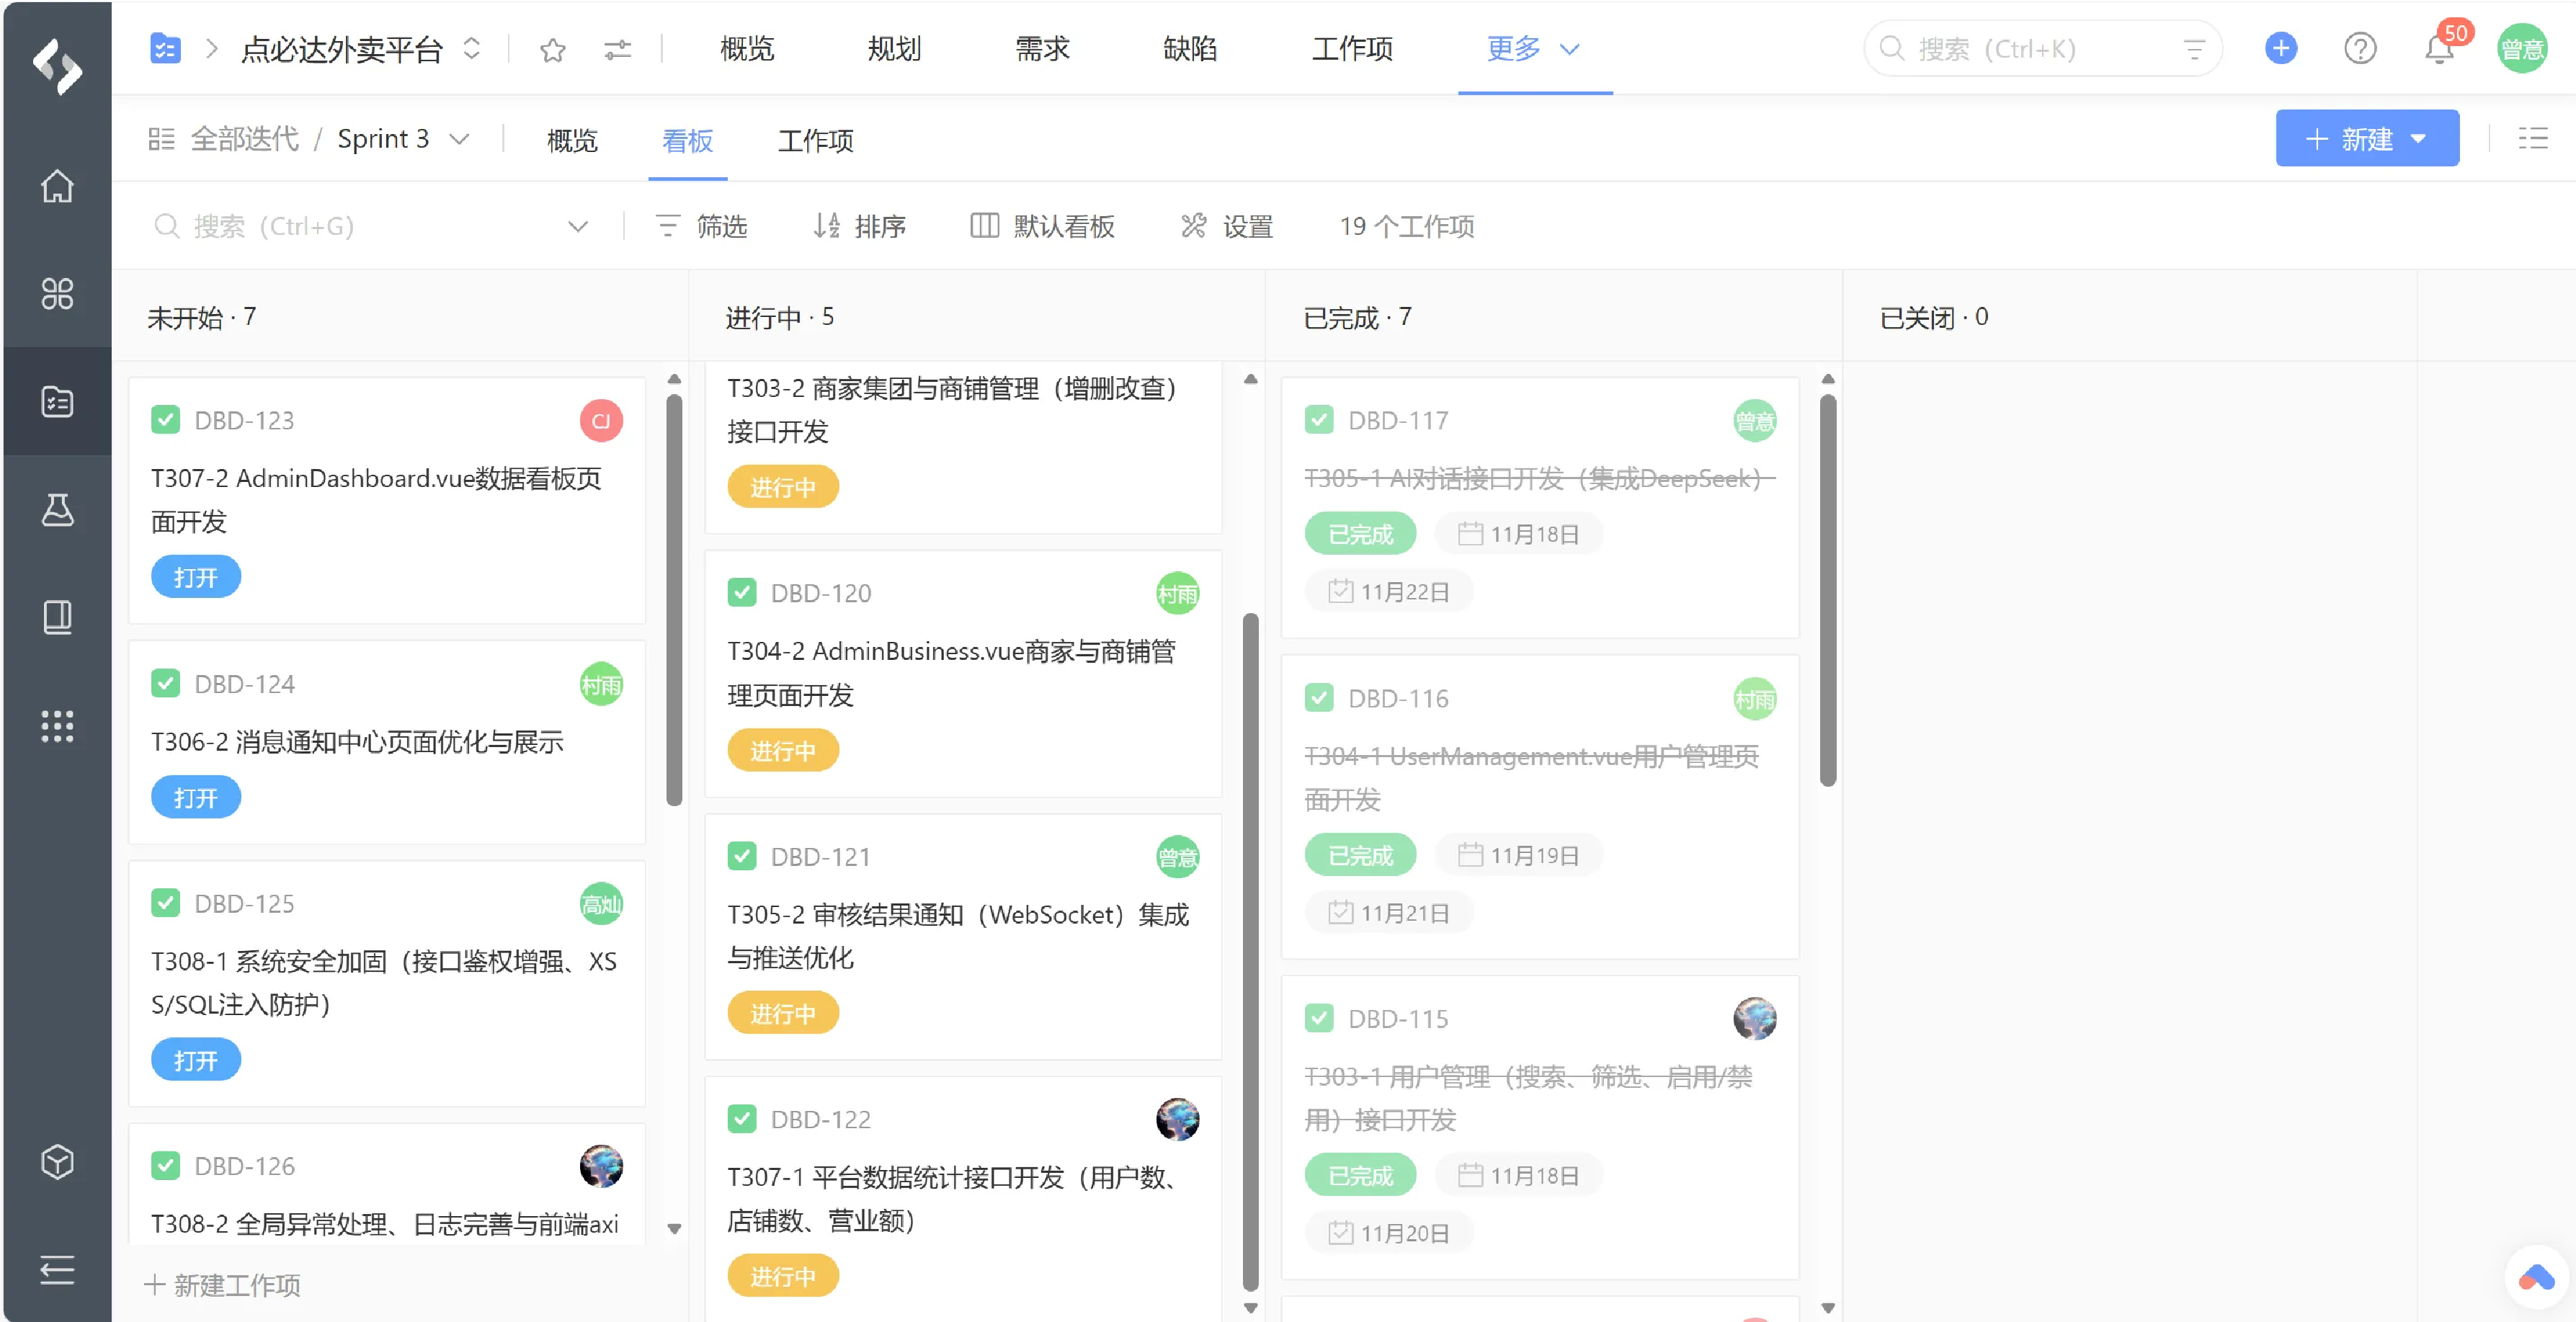
\includegraphics[width=1\textwidth]{figures/in/image3}
                  \caption{Sprint3燃尽图数据来源}
              \end{figure}

        \item \textbf{燃尽图图表}
              \begin{figure}[H]
                  \centering
                  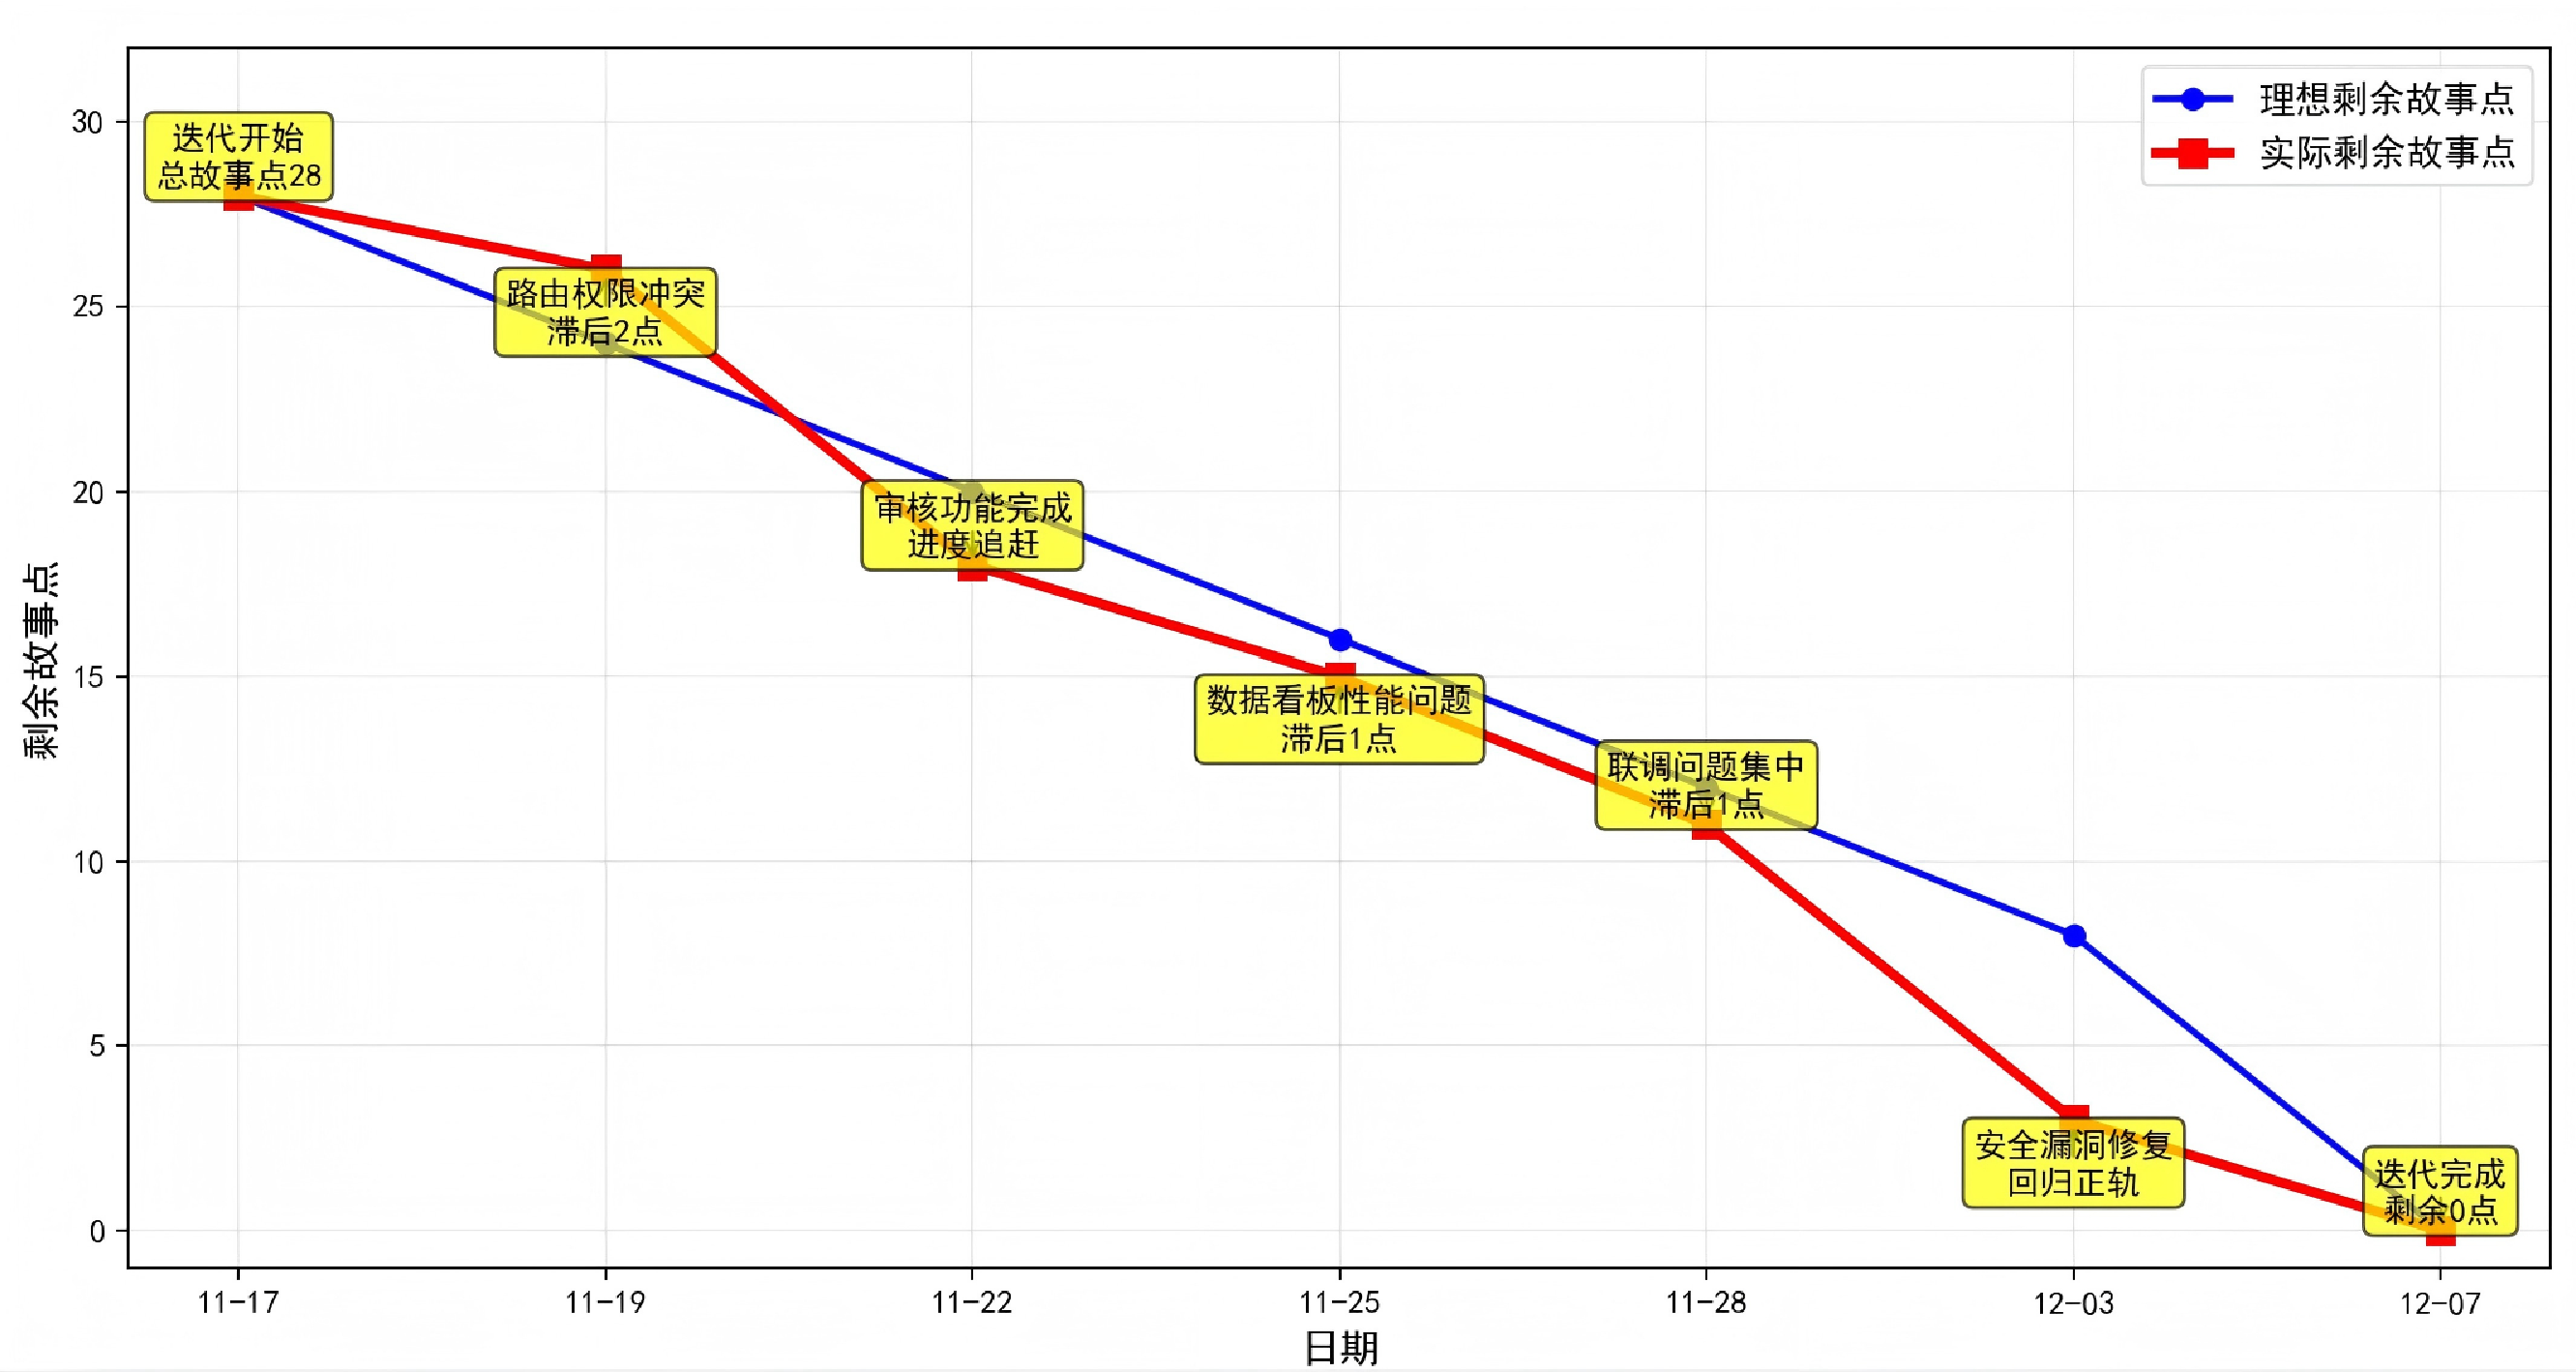
\includegraphics[width=1\textwidth]{figures/in/fire3}
                  \caption{Sprint3燃尽图 (11.17-12.7)}
              \end{figure}


        \item \textbf{进度偏差分析}
              \begin{itemize}
                  \item 偏差点 1（11.19）
                        \begin{itemize}
                            \item 偏差情况：管理员路由权限与现有用户系统冲突，T304-1（UserManagement.vue 用户管理页面开发）和 T301-2（商铺审核接口开发）均受阻，延误 2 小时。
                            \item 影响分析：管理端核心页面与接口开发滞后，可能导致后续联调时间压缩，影响审核功能整体进度。
                            \item 解决方案：Scrum Master 高灿组织前后端协作，前端在路由守卫中增加角色判断逻辑，后端通过路径区分 /admin/（管理员接口）与 /api/（普通接口），明确权限校验边界。
                            \item 偏差量：约 0.5 个故事点
                        \end{itemize}

                  \item 偏差点 2（11.25）
                        \begin{itemize}
                            \item 偏差情况：T307-2（AdminDashboard.vue 数据看板开发）中统计查询接口响应缓慢，页面加载延迟超 3 秒，开发暂停。
                            \item 影响分析：数据看板作为管理端核心功能，性能不达标将影响管理员决策效率，需优先优化。
                            \item 解决方案：戴茗静为用户数、店铺数、营业额等统计查询添加数据库联合索引，优化 SQL 查询逻辑，减少冗余计算，将响应时间压缩至 1 秒内。
                            \item 偏差量：约 0.5 个故事点
                        \end{itemize}

                  \item 偏差点3（11.27）
                        \begin{itemize}
                            \item 偏差情况：T306-1（AIChat.vue 智能助手页面）与后端 AI 接口联调时，因接口响应格式与前期约定不一致，开发受阻 3 小时。
                            \item 影响分析：AI 客服作为核心增值功能，联调滞后将影响用户体验测试，无法验证 “响应时间 < 3 秒” 的验收标准。
                            \item 解决方案：曾意提供标准化接口响应示例文档，明确用户消息、AI 回答、会话 ID 等字段格式，贾思韵调整前端数据解析逻辑，同步完成联调与响应时间优化。
                            \item 偏差量：约 0.5 个故事点
                        \end{itemize}

                  \item 偏差点4（11.28）
                        \begin{itemize}
                            \item 偏差情况：集成联调阶段发现 3 个关键问题：AI 聊天图片上传失败、数据看板数字显示格式错误、用户禁用后缓存未清理，导致联调进度滞后 4 小时。
                            \item 影响分析：多模块并行问题集中暴露，若未及时修复将影响专项测试启动时间，可能导致迭代延期。
                            \item 解决方案：按模块分配修复责任人 —— 曾意修复 AI 图片上传接口适配问题，杨晓越修正数字格式化逻辑，高灿通过添加缓存失效机制解决用户状态同步问题，同步开展回归验证。
                            \item 偏差量：约 1 个故事点
                        \end{itemize}

                  \item 偏差点 5（12.03）
                        \begin{itemize}
                            \item 偏差情况：专项测试中发现 2 个安全漏洞（越权访问潜在风险），涉及管理员接口权限校验不严谨，需紧急修复。
                            \item 影响分析：安全漏洞直接违反 US019（系统安全）验收标准，若未修复将导致迭代验收不通过，存在数据泄露风险。
                            \item 解决方案：高灿紧急强化接口权限校验，为所有管理员接口添加角色注解与拦截器双重校验，任晓华针对漏洞场景编写专项测试用例，复测通过后才进入预部署阶段。
                            \item 偏差量：约 0.5 个故事点
                        \end{itemize}

              \end{itemize}

    \end{enumerate}

\end{levellist}
